%%%%%%%%%%%%%%%%%%%%%%%%%%%%%%%%%%%%%%%%%
% Beamer Presentation
% LaTeX Template
% Version 1.0 (10/11/12)
%
% This template has been downloaded from:
% http://www.LaTeXTemplates.com
%
% License:
% CC BY-NC-SA 3.0 (http://creativecommons.org/licenses/by-nc-sa/3.0/)
%
%%%%%%%%%%%%%%%%%%%%%%%%%%%%%%%%%%%%%%%%%

%----------------------------------------------------------------------------------------
%	PACKAGES AND THEMES
%----------------------------------------------------------------------------------------

\documentclass{beamer}

\mode<presentation> {

% The Beamer class comes with a number of default slide themes
% which change the colors and layouts of slides. Below this is a list
% of all the themes, uncomment each in turn to see what they look like.

%\usetheme{default}
%\usetheme{AnnArbor}
%\usetheme{Antibes}
%\usetheme{Bergen}
%\usetheme{Berkeley}
%\usetheme{Berlin}
%\usetheme{Boadilla}
%\usetheme{CambridgeUS}
%\usetheme{Copenhagen}
%\usetheme{Darmstadt}
%\usetheme{Dresden}
%\usetheme{Frankfurt}
%\usetheme{Goettingen}
%\usetheme{Hannover}
%\usetheme{Ilmenau}
%\usetheme{JuanLesPins}
%\usetheme{Luebeck}
\usetheme{Madrid}
%\usetheme{Malmoe}
%\usetheme{Marburg}
%\usetheme{Montpellier}
%\usetheme{PaloAlto}
%\usetheme{Pittsburgh}
%\usetheme{Rochester}
%\usetheme{Singapore}
%\usetheme{Szeged}
%\usetheme{Warsaw}

% As well as themes, the Beamer class has a number of color themes
% for any slide theme. Uncomment each of these in turn to see how it
% changes the colors of your current slide theme.

%\usecolortheme{albatross}
%\usecolortheme{beaver}
%\usecolortheme{beetle}
%\usecolortheme{crane}
%\usecolortheme{dolphin}
%\usecolortheme{dove}
%\usecolortheme{fly}
%\usecolortheme{lily}
%\usecolortheme{orchid}
%\usecolortheme{rose}
%\usecolortheme{seagull}
%\usecolortheme{seahorse}
%\usecolortheme{whale}
%\usecolortheme{wolverine}

%\setbeamertemplate{footline} % To remove the footer line in all slides uncomment this line
%\setbeamertemplate{footline}[page number] % To replace the footer line in all slides with a simple slide count uncomment this line

%\setbeamertemplate{navigation symbols}{} % To remove the navigation symbols from the bottom of all slides uncomment this line
}

\usepackage{graphicx} % Allows including images
\usepackage{booktabs} % Allows the use of \toprule, \midrule and \bottomrule in tables
\usepackage[export]{adjustbox}
\usepackage{listings}
%----------------------------------------------------------------------------------------
%	TITLE PAGE
%----------------------------------------------------------------------------------------

\title[BobKonf]{ImplicitCAD: Haskell all of the Things} % The short title appears at the bottom of every slide, the full title is only on the title page

\author{Julia Longtin} % Your name
\institute[ImplicitCAD] % Your institution as it will appear on the bottom of every slide, may be shorthand to save space
{
ImplicitCAD Project \\ % Your institution for the title page
\medskip
\textit{julia.longtin@gmail.com} % Your email address
}
\date{\today} % Date, can be changed to a custom date

% disable page count
\setbeamertemplate{page number in head/foot}{}

\begin{document}

\begin{frame}
\titlepage % Print the title page as the first slide
\begin{block}{Source to this talk}
\begin{itemize}
\item https://github.com/julialongtin/BobKonf2020.git
\end{itemize}
\end{block}
\end{frame}

%\begin{frame}
%\frametitle{Overview} % Table of contents slide, comment this block out to remove it
%\tableofcontents % Throughout your presentation, if you choose to use \section{} and \subsection{} commands, these will automatically be printed on this slide as an overview of your presentation
%\end{frame}

%----------------------------------------------------------------------------------------
%	PRESENTATION SLIDES
%----------------------------------------------------------------------------------------

%------------------------------------------------
\section{Who Am I?} % Sections can be created in order to organize your presentation into discrete blocks, all sections and subsections are automatically printed in the table of contents as an overview of the talk
%------------------------------------------------

\begin{frame}
\frametitle{Who am I?}
\begin{itemize}
\item Free Software Developer for 20+ years
  \begin{itemize}
  \item Contributor to OpenEMR, FAI, TinTin++, LinuxPMI,...
  \end{itemize}
\item Work at Wire.com
  \begin{itemize}
  \item The presented work has no affiliation with my employer
  \end{itemize}
\item Maintainer of ImplicitCAD
\item Author of HSlice
\end{itemize}
\end{frame}

%------------------------------------------------

\begin{frame}
\frametitle{Who am I?}
\begin{itemize}
\item Have run two Hackerspaces
\end{itemize}
\begin{columns}
  \begin{column}{0.5\textwidth}
    
\includegraphics[width=0.5\textwidth, right]{HacDC.svg.png}
  \end{column}
  \begin{column}{0.5\textwidth}
    
\includegraphics[width=0.5\textwidth, left]{FreeGeekLogo.png}
  \end{column}
\end{columns}
\begin{itemize}
\item Spent 8+ years teaching 10 hours a week
\item Tested ImplicitCAD on the members at HacDC
\end{itemize}
\end{frame}

\begin{frame}
\frametitle{Who am I?}
\begin{itemize}
\item Transhumanist, 3D printer aficionado
\begin{itemize}
\item ... would love to be bio-printing ...
\end{itemize}
\item Scratch building mutant printers for 10+ years
\item Created method for converting 3D prints to aluminium with microwaves (see: 31c3)
\end{itemize}
\end{frame}

%------------------------------------------------

\section{ImplicitCAD Overview}

\subsection{General Description}
\begin{frame}
\frametitle{What is ImplicitCAD?}
\begin{itemize}
\item Programmatic 3D Modeling System
\item Originally written by Christopher Olah in 2011
  \begin{itemize}
  \item I took over as maintainer in 2014
  \end{itemize}
\item Licensed under the AGPLv3+
\item Written in Haskell
\end{itemize}
\begin{block}{Source Code}
\begin{itemize}
\item https://github.com/colah/ImplicitCAD/
\end{itemize}
\end{block}
\begin{block}{Online Editor}
\begin{itemize}
\item http://implicitcad.org/editor/
\end{itemize}
\end{block}
\end{frame}

\begin{frame}
\frametitle{What is ImplicitCAD?}
\begin{itemize}
\item Three Components:
  \begin{itemize}
  \item 3D/2D Rendering Engine
  \item SCAD Execution Engine
  \item Library (Haskell DSL)
  \end{itemize}
\end{itemize}
\end{frame}

%------------------------------------------------

\subsection{Rendering Engine}
\begin{frame}
\frametitle{ImplicitCAD's Rendering Engine}
\begin{itemize}
\item Renders 3D: STL, OBJ... ``Triangles on the outside''.
\begin{itemize}
\item Uses marching cubes algorithm for triangulation functions
\end{itemize}
\item Renders 2D: SVG, SCAD, PNG, DXF...
\begin{itemize}
\item Uses modified marching squares, or ray tracing depending on format
\end{itemize}
\end{itemize}
\begin{columns}
  \begin{column}{0.33\textwidth}
    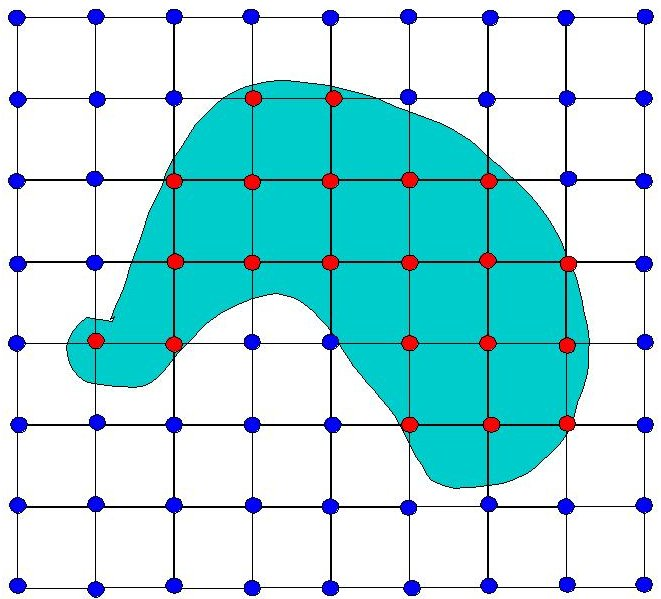
\includegraphics[width=0.8\textwidth, right]{labeledobj.jpg}
  \end{column}
  \begin{column}{0.33\textwidth}
    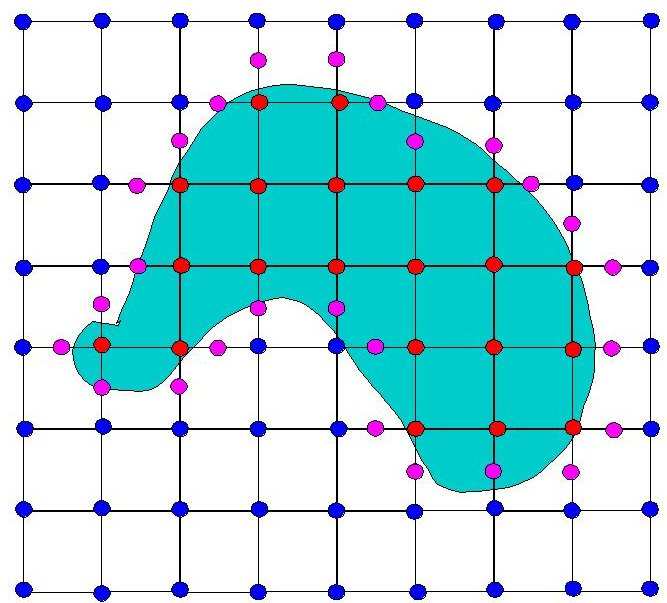
\includegraphics[width=0.8\textwidth, center]{purpledobj.jpg}
  \end{column}
  \begin{column}{0.33\textwidth}
    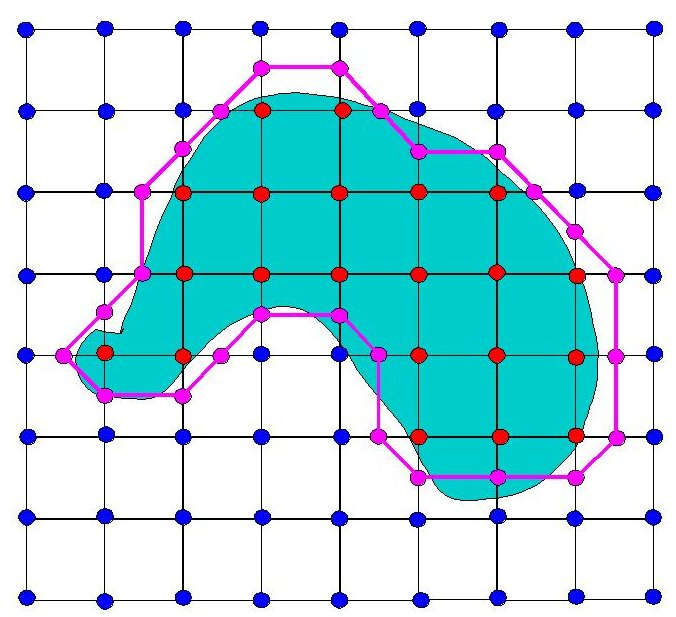
\includegraphics[width=0.8\textwidth, left]{connectedobj.jpg}
  \end{column}
\end{columns}
\begin{itemize}
\item Highly parallelized, uses all CPUs
\end{itemize}
\end{frame}

\subsection{Scad Execution Engine}
\begin{frame}[fragile]
\frametitle{ImplicitCAD's SCAD Execution Engine}
\begin{itemize}
\item OpenSCAD like, not quite OpenSCAD compatible
\begin{itemize}
\item Lack of a real SCAD standard allows us to experiment with the language
\end{itemize}
\item Leans toward primitive elements with more power
\end{itemize}
\begin{columns}
  \begin{column}{0.5\textwidth}
  \lstset{basicstyle=\ttfamily\scriptsize}
\begin{lstlisting}
  cylinder(h=1,r=10);
\end{lstlisting}
    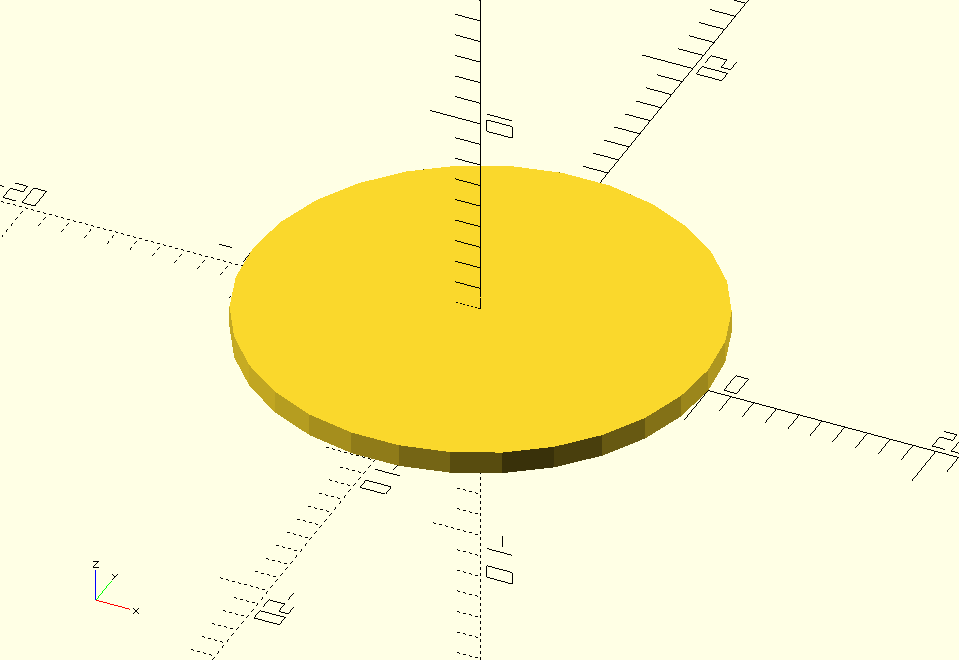
\includegraphics[width=0.9\textwidth, left]{openscad-cylinder.png}
  \end{column}
  \begin{column}{0.5\textwidth}
  \lstset{basicstyle=\ttfamily\scriptsize}
\begin{lstlisting}
  cylinder(h=1,r=10);
\end{lstlisting}
    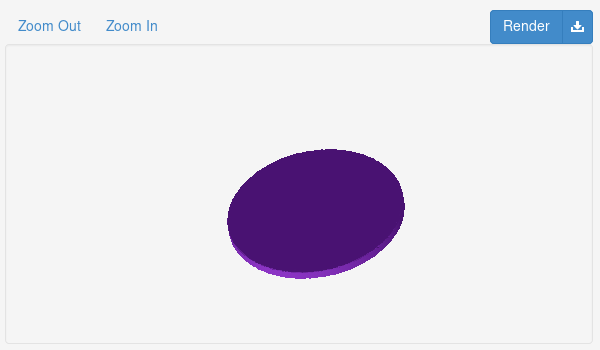
\includegraphics[width=0.9\textwidth, right]{implicitcad-cylinder.png}
  \end{column}
\end{columns}
\end{frame}

\subsection{Library}
\begin{frame}
\frametitle{ImplicitCAD's Haskell Library}
\begin{itemize}
\item Usable from simple Haskell programs (Haskell DSL!) to generate objects
\item Capable of SCAD execution without modeling
\item Separable expression executor
\end{itemize}
\end{frame}

\subsection{Executables}
\begin{frame}
\frametitle{ImplicitCAD Executables}
\begin{itemize}
\item extopenscad: SCAD engine in command line form
\end{itemize}
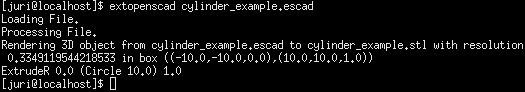
\includegraphics[width=1.0\textwidth, left]{extopenscad_example.png}
\begin{itemize}
\item ImplicitSNAP: Engine backing the web site.
\end{itemize}
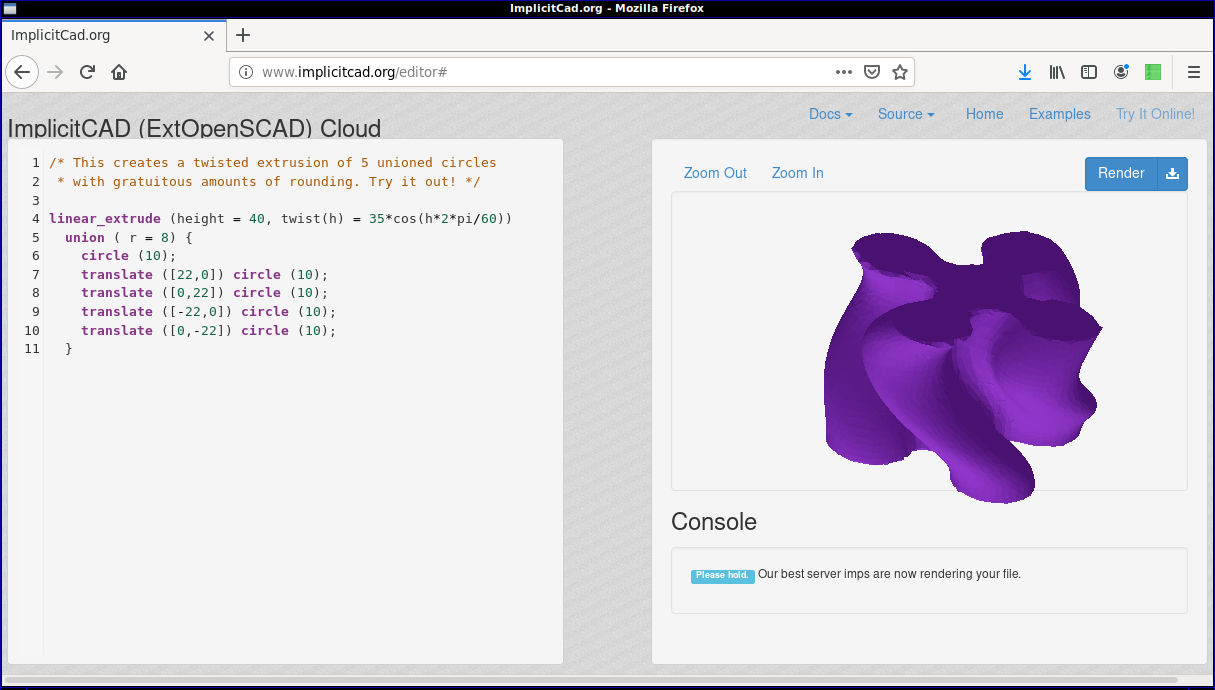
\includegraphics[width=0.6\textwidth, center]{website-frame_grab.png}
\end{frame}

\section{Other SCAD Engines}
\begin{frame}
\frametitle{Other SCAD Engines}
\begin{block}{OpenSCAD - https://openscad.org}
\begin{itemize}
\item Graphical Interface
\item Written in C++
\item GPLv2 License
\end{itemize}
\end{block}
\begin{block}{OpenJSCAD - https://openjscad.org}
\begin{itemize}
\item Web based User Interface
\item Writen in JavaScript
\item MIT License
\end{itemize}
\end{block}
\end{frame}

\begin{frame}
\frametitle{Other SCAD Engines}
\begin{block}{Curv - https://curv3d.org}
\begin{itemize}
\item Graphical Interface, GPU required
\item Apache License
\item Written in C++
\item Uses maths based on ImplicitCAD
\end{itemize}
\end{block}
\begin{block}{CadQuery - https://github.com/CadQuery/cadquery}
\begin{itemize}
\item Graphical Interface, GPU required
\item Apache License
\item Python based
\end{itemize}
\end{block}
\end{frame}

\begin{frame}
\frametitle{Other Python SCAD engines?}
\begin{itemize}
\item At least three rewrites of ImplicitCAD in Python
\begin{itemize}
\item All Non-Free, one in use by military...
\end{itemize}
\end{itemize}
\end{frame}

\section{Why ImplicitCAD?}
\begin{frame}
  \frametitle{Why ImplicitCAD?}
\begin{itemize}
\item Simple SCAD Language
\end{itemize}
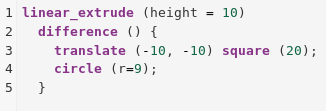
\includegraphics[width=0.5\textwidth, center]{website-simple_example_text.png}

\includegraphics[width=0.5\textwidth, center]{website-simple_example_graphic.png}
\end{frame}

\begin{frame}[fragile]
  \frametitle{Why ImplicitCAD?}
  \lstset{basicstyle=\ttfamily\scriptsize}
\begin{itemize}
\item Simple Haskell DSL
\end{itemize}
\begin{lstlisting}
  -- A simple cylinder
  import Prelude (($))
  import Graphics.Implicit(writeSTL, cylinder2)

  main = writeSTL 0.2 ``cylinder_example.stl'' $ cylinder2 10 10 1
\end{lstlisting}
    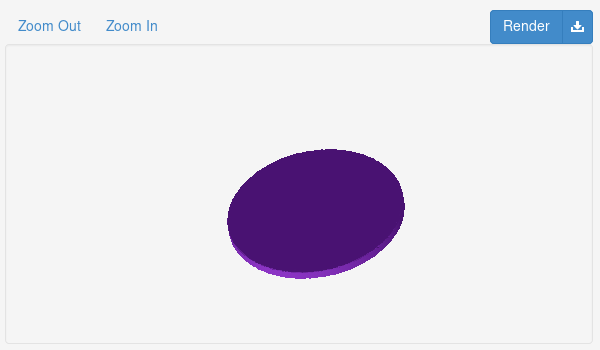
\includegraphics[width=0.7\textwidth, center]{implicitcad-cylinder.png}
\end{frame}

\begin{frame}[fragile]
  \frametitle{Why ImplicitCAD?}
\begin{itemize}
\item Nearly Haskell-Native intermediate state
\end{itemize}
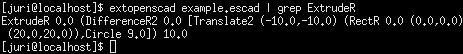
\includegraphics[width=1.0\textwidth, center]{extopenscad-haskell_intermediate.png}
\lstset{basicstyle=\ttfamily\scriptsize}
\begin{lstlisting}
  -- A simple cylinder
  import Prelude (($))
  import Graphics.Implicit

  main = writeSTL 0.2 ``example.stl'' $
    extrudeR 0.0 (differenceR 0.0 [translate (-10.0,-10.0) $
                  rectR 0.0 (0.0,0.0) (20.0,20.0),
                  circle 9.0]) 10.0
\end{lstlisting}
\end{frame}

\begin{frame}
  \frametitle{Why ImplicitCAD?}
\begin{itemize}
\item Implicit Constructive Solid Geometry
\end{itemize}
\begin{columns}
  \begin{column}{0.5\textwidth}
    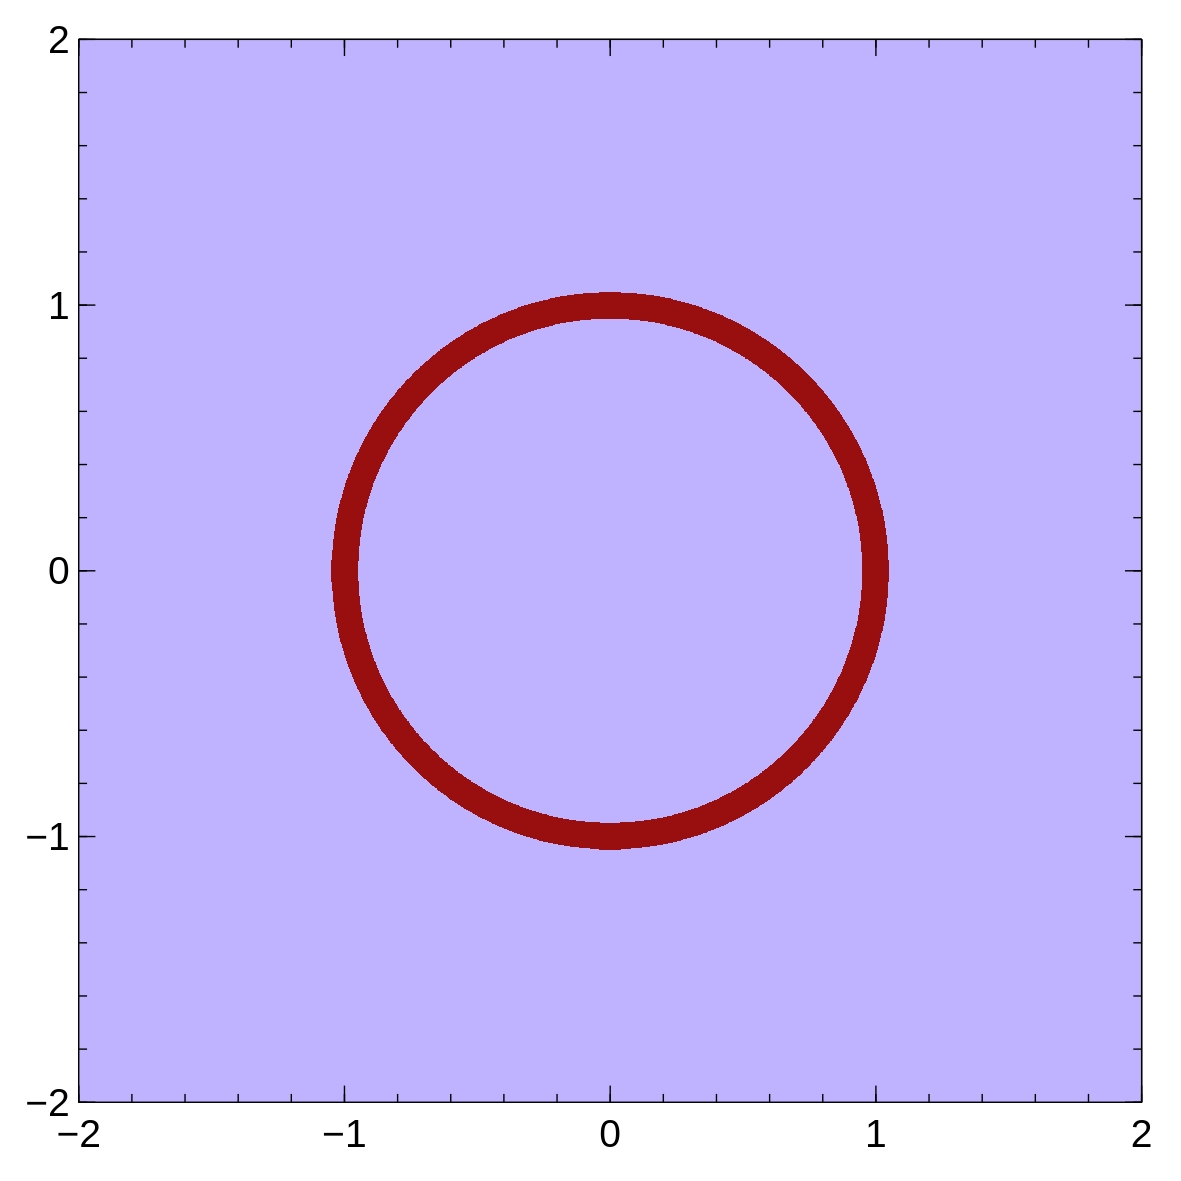
\includegraphics[width=1.0\textwidth, left]{normal_circle.jpg}
  \end{column}
  \begin{column}{0.5\textwidth}
    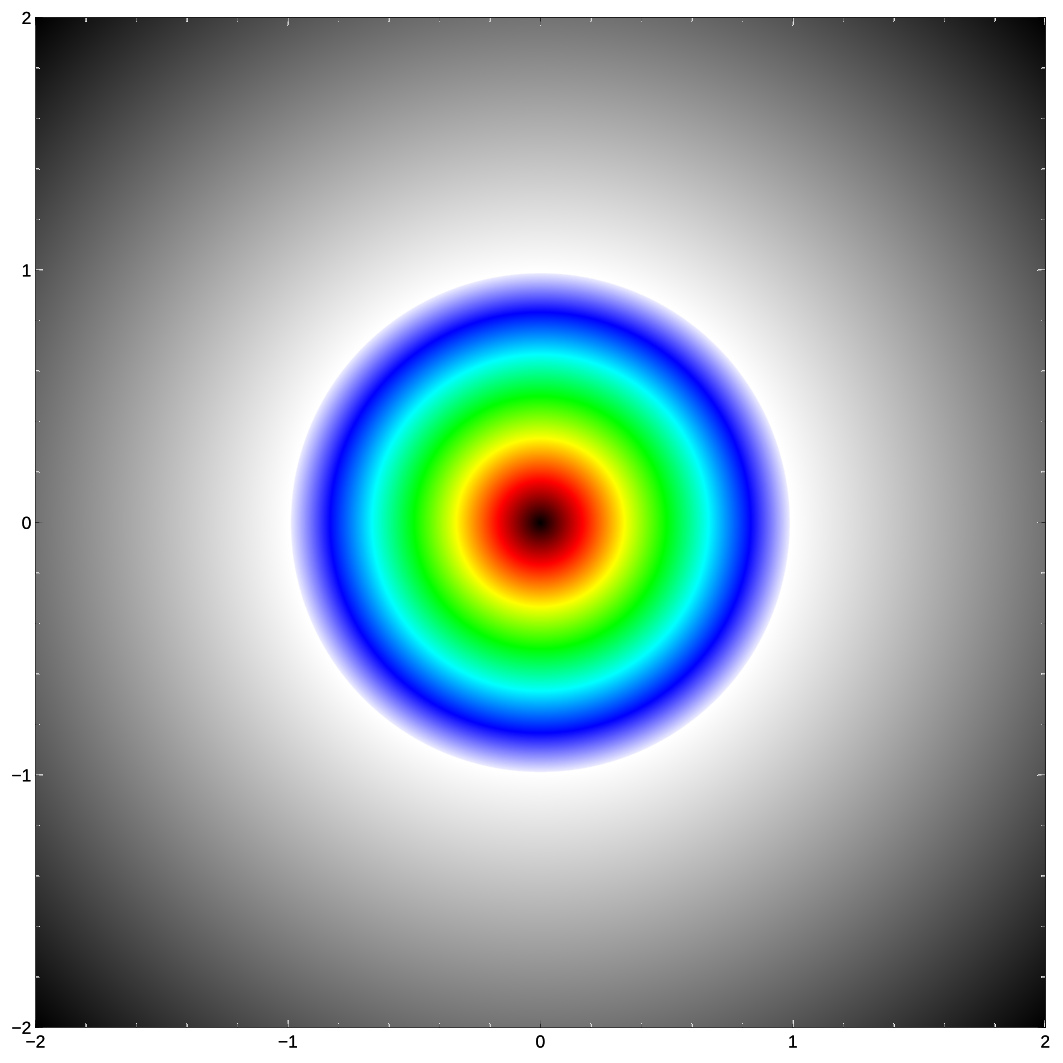
\includegraphics[width=1.0\textwidth, right]{implicit_circle.jpg}
  \end{column}
\end{columns}
\end{frame}

\begin{frame}
\frametitle{Why ImplicitCAD?}
\begin{itemize}
\item High Performance through parallel list comprehensions
\end{itemize}
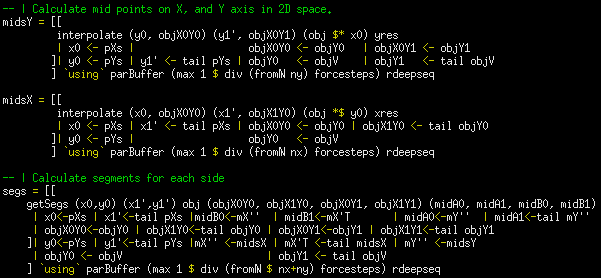
\includegraphics[width=1.0\textwidth, left]{2D_renderer.png}
\end{frame}

\section{CSG in SCAD}

\begin{frame}
\frametitle{Basic CSG in SCAD}
\begin{columns}
  \begin{column}{0.5\textwidth}
    \begin{itemize}
    \item circle(r=9);
    \end{itemize}
  \end{column}
  \begin{column}{0.5\textwidth}
    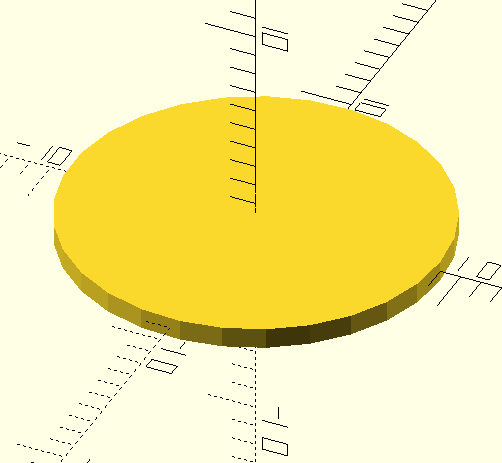
\includegraphics[width=0.5\textwidth, right]{openscad-circle_9.png}
  \end{column}
\end{columns}
\begin{columns}
  \begin{column}{0.5\textwidth}
    \begin{itemize}
    \item square(20);
    \end{itemize}
  \end{column}
  \begin{column}{0.5\textwidth}
    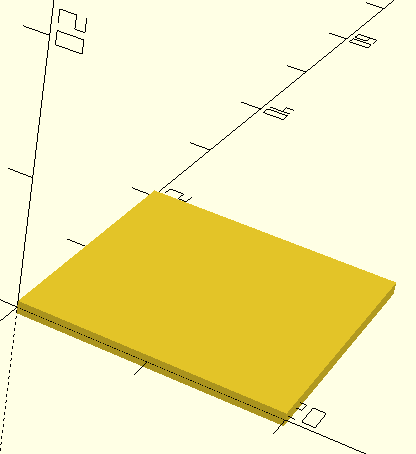
\includegraphics[width=0.5\textwidth, right]{openscad-square_20.png}
  \end{column}
\end{columns}
\end{frame}

\begin{frame}
\frametitle{Basic CSG in SCAD}
\begin{columns}
  \begin{column}{0.5\textwidth}
    \begin{itemize}
    \item translate([-10,-10]) square(20); 
    \end{itemize}
  \end{column}
  \begin{column}{0.5\textwidth}
    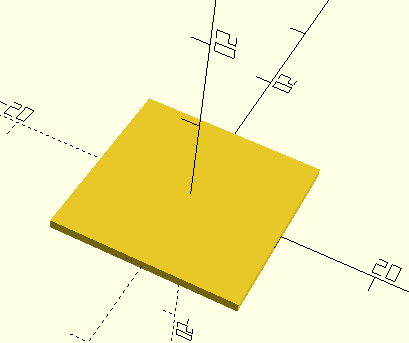
\includegraphics[width=0.5\textwidth, right]{openscad-translate_square_20.png}
  \end{column}
\end{columns}
\begin{columns}
  \begin{column}{0.5\textwidth}
    \begin{itemize}
    \item union() \{ circle(r=9); square(20); \}
    \end{itemize}
  \end{column}
  \begin{column}{0.5\textwidth}
    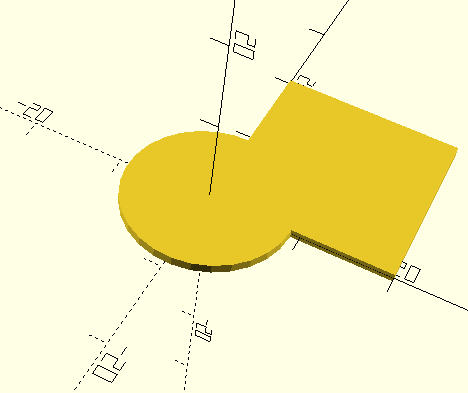
\includegraphics[width=0.5\textwidth, right]{openscad-union_circle_9_square_20.png}
  \end{column}
\end{columns}
\end{frame}

\begin{frame}
\frametitle{Basic CSG in SCAD}
\begin{columns}
  \begin{column}{0.5\textwidth}
    \begin{itemize}
    \item intersection() \{ circle(r=9); square(20); \} 
    \end{itemize}
  \end{column}
  \begin{column}{0.5\textwidth}
    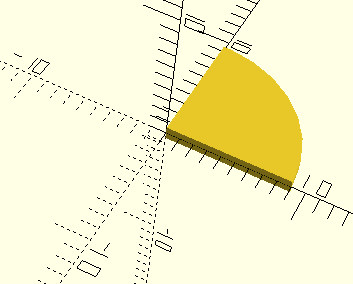
\includegraphics[width=0.5\textwidth, right]{openscad-intersection_circle_9_square_20.png}
  \end{column}
\end{columns}
\begin{columns}
  \begin{column}{0.5\textwidth}
    \begin{itemize}
    \item difference() \{ circle(r=9); square(20); \}
    \end{itemize}
  \end{column}
  \begin{column}{0.5\textwidth}
    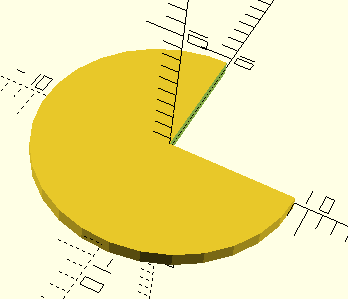
\includegraphics[width=0.5\textwidth, right]{openscad-difference_circle_9_square_20.png}
  \end{column}
\end{columns}
\end{frame}

\section{CSG in Haskell}

\begin{frame}
\frametitle{Basic CSG in Haskell}
\begin{columns}
  \begin{column}{0.5\textwidth}
    \begin{itemize}
    \item main = writeSVG 0.2 ``example.svg'' \$ circle 9.0
    \end{itemize}
  \end{column}
  \begin{column}{0.5\textwidth}
    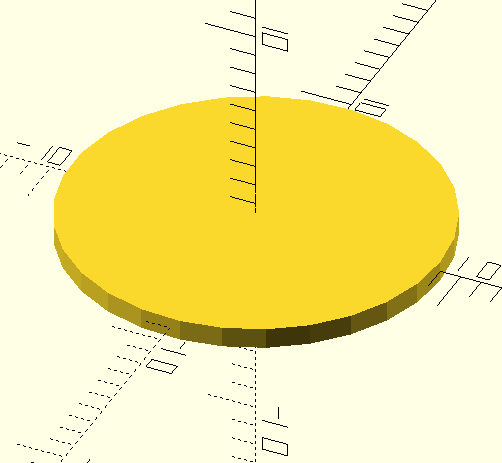
\includegraphics[width=0.5\textwidth, right]{openscad-circle_9.png}
  \end{column}
\end{columns}
\begin{columns}
  \begin{column}{0.5\textwidth}
    \begin{itemize}
    \item main = writeSVG 0.2 ``example.svg'' \$ rectR 0 (0,0) (20,20)
    \end{itemize}
  \end{column}
  \begin{column}{0.5\textwidth}
    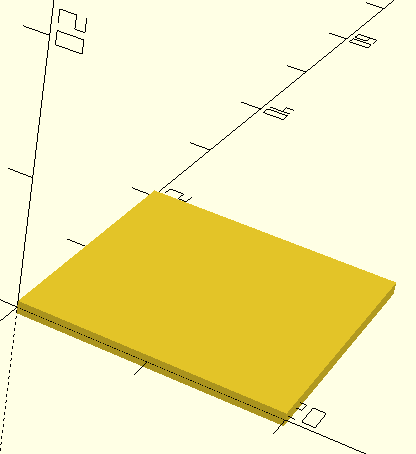
\includegraphics[width=0.5\textwidth, right]{openscad-square_20.png}
  \end{column}
\end{columns}
\end{frame}

\begin{frame}
\frametitle{Basic CSG in Haskell}
\begin{columns}
  \begin{column}{0.5\textwidth}
    \begin{itemize}
    \item main = writeSVG 0.2 ``example.svg'' \$ translate (-10,-10) \$ rectR 0 (0,0) (20,20)
    \end{itemize}
  \end{column}
  \begin{column}{0.5\textwidth}
    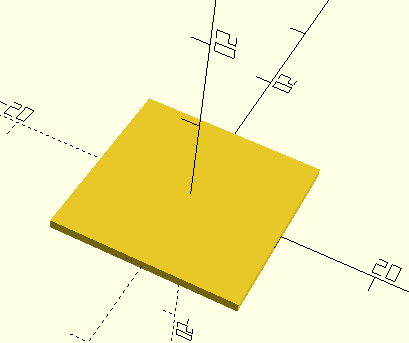
\includegraphics[width=0.5\textwidth, right]{openscad-translate_square_20.png}
  \end{column}
\end{columns}
\begin{columns}
  \begin{column}{0.5\textwidth}
    \begin{itemize}
    \item main = writeSVG 0.2 ``example.svg'' \$ unionR 0 [circle 9, rectR 0 (0,0) (20,20)]
    \end{itemize}
  \end{column}
  \begin{column}{0.5\textwidth}
    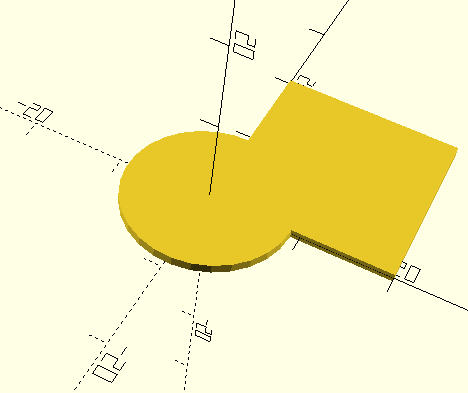
\includegraphics[width=0.5\textwidth, right]{openscad-union_circle_9_square_20.png}
  \end{column}
\end{columns}
\end{frame}

\begin{frame}
\frametitle{Basic CSG in Haskell}
\begin{columns}
  \begin{column}{0.5\textwidth}
    \begin{itemize}
    \item main = writeSVG 0.2 ``example.svg'' \$ intersectR 0 [circle 9, rectR 0 (0,0) (20,20)]
    \end{itemize}
  \end{column}
  \begin{column}{0.5\textwidth}
    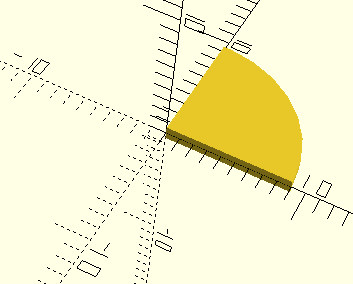
\includegraphics[width=0.5\textwidth, right]{openscad-intersection_circle_9_square_20.png}
  \end{column}
\end{columns}
\begin{columns}
  \begin{column}{0.5\textwidth}
    \begin{itemize}
    \item main = writeSVG 0.2 ``example.svg'' \$ differenceR 0 [circle 9, rectR 0 (0,0) (20,20)]
    \end{itemize}
  \end{column}
  \begin{column}{0.5\textwidth}
    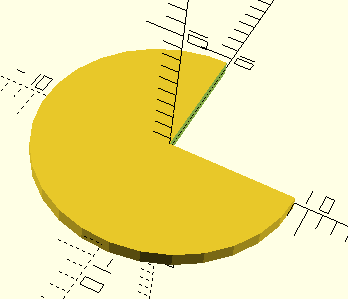
\includegraphics[width=0.5\textwidth, right]{openscad-difference_circle_9_square_20.png}
  \end{column}
\end{columns}
\end{frame}

\begin{frame}
\frametitle{Additional Primitives}
\begin{itemize}
\item polygon();
\item cube();
\item sphere();
\item cylinder();
\end{itemize}
\end{frame}

\begin{frame}
\frametitle{Additional Operations}
\begin{itemize}
\item scale() \{ \}
\item rotate() \{ \}
\item linear\_extrude( ) \{ \}
\end{itemize}
\end{frame}

\begin{frame}
\frametitle{Flow Control}
\begin{itemize}
\item module ( ) \{ \}
\item function ( ) ...
\item if ... then ... else
\item for ( ) \{ \}
\item include ...
\item use ...
\item echo ();
\end{itemize}
\end{frame}

\section{SCAD Examples}
\begin{frame}[fragile]
\frametitle{SCAD Example: Disc}
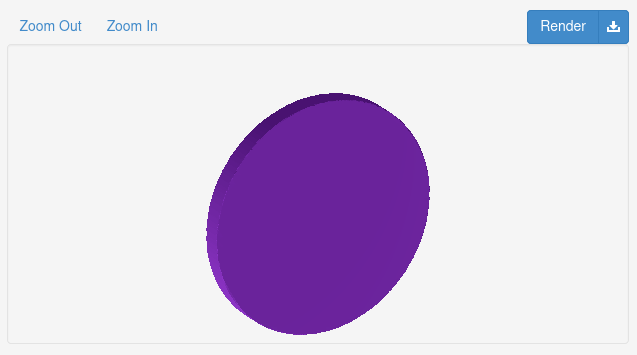
\includegraphics[width=0.5\textwidth, center]{disc_example.png}
  \lstset{basicstyle=\ttfamily\scriptsize}
    \begin{lstlisting}
    module disc_2d(diameter){
      radius=diameter/2;
      circle(r=radius);
    }
    module disc_3d(diameter, thickness){
      linear_extrude(thickness)
      disc_2d(diameter);
    }
    disc_3d(thickness=10, diameter=120);
    \end{lstlisting}
\end{frame}

\begin{frame}[fragile]
\frametitle{SCAD Example: Bead}
\lstset{basicstyle=\ttfamily\scriptsize}
\begin{columns}
  \begin{column}{0.2\textwidth}
    
\includegraphics[width=1.0\textwidth, center]{bead_example.png}
  \end{column}
  \begin{column}{0.8\textwidth}
    \begin{lstlisting}
      module bead_3d(height,diameter,hole_diameter) {
        difference() {
          cylinder(r=diameter/2, h=height);
          cylinder(r=hole_diameter/2, h=height);
        }
      }
      bead_3d(height=10, diameter=120,hole_diameter=20);
    \end{lstlisting}
  \end{column}
\end{columns}
\end{frame}

\section{Implicit CSG}
\begin{frame}[fragile]
\frametitle{Implicit CSG}
\begin{itemize}
\item CSG using Implicit functions
\item Implicit functions are functions that define gradient to edge
\item Interior of objects = negative value
\item Exterior of objects = positive value
\end{itemize}
\end{frame}

\begin{frame}
\frametitle{Circles}
\begin{columns}
  \begin{column}{0.5\textwidth}
    \begin{itemize}
    \item $x^2+y^2=r^2$
    \end{itemize}
  \end{column}
  \begin{column}{0.5\textwidth}
    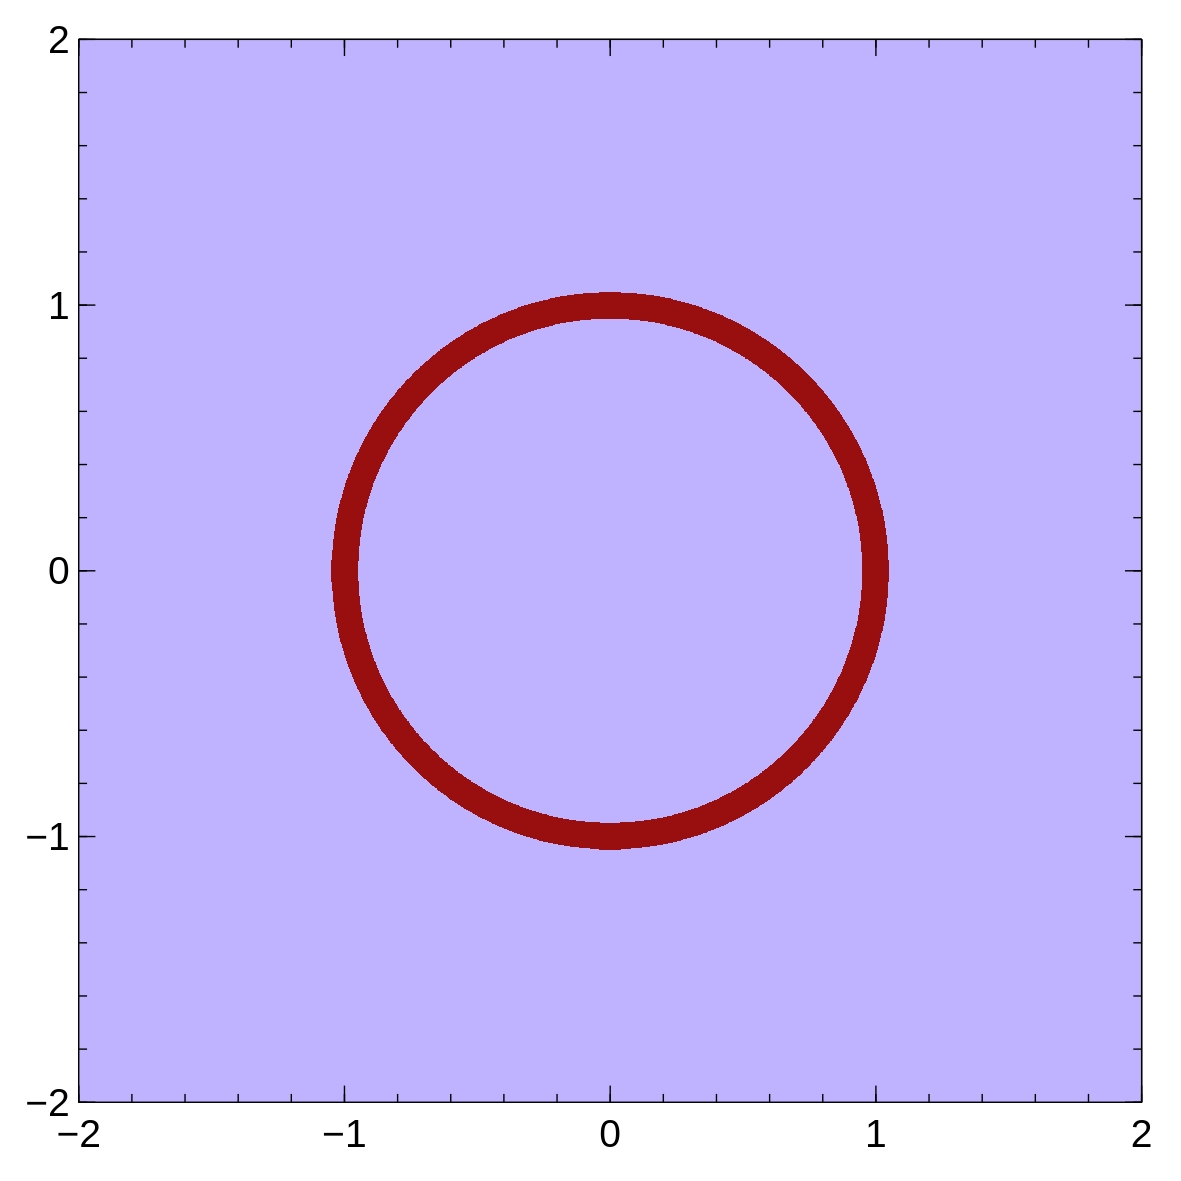
\includegraphics[width=0.5\textwidth, right]{normal_circle.jpg}
  \end{column}
\end{columns}
\begin{columns}
  \begin{column}{0.5\textwidth}
    \begin{itemize}
    \item $f(x,y)=sqrt(x^2+y^2)-1$
    \end{itemize}
  \end{column}
  \begin{column}{0.5\textwidth}
    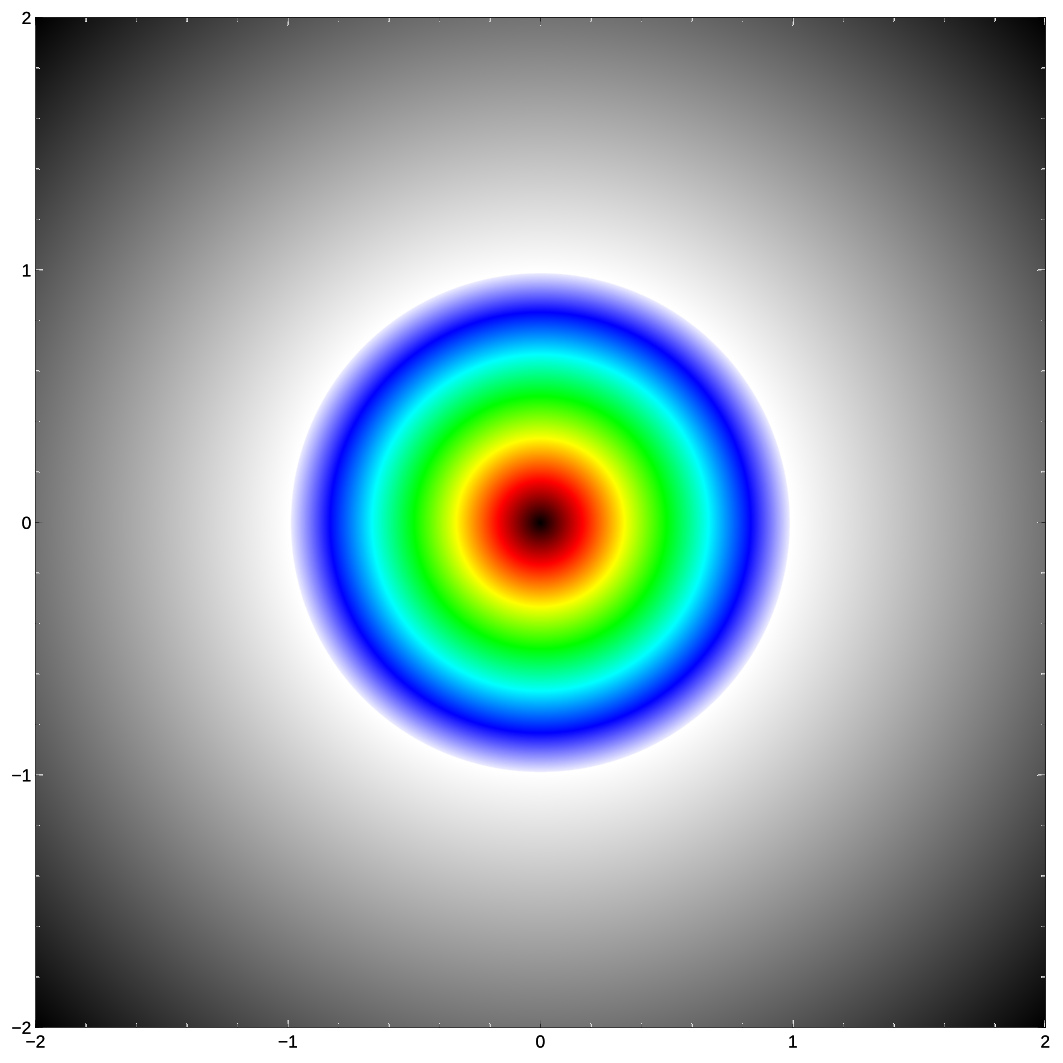
\includegraphics[width=0.5\textwidth, right]{implicit_circle.jpg}
  \end{column}
\end{columns}
\end{frame}

\begin{frame}
\frametitle{Translation}
\begin{columns}
  \begin{column}{0.5\textwidth}
    \begin{itemize}
    \item $f(x,y)=sqrt(x^2+y^2)-1$
    \end{itemize}
  \end{column}
  \begin{column}{0.5\textwidth}
    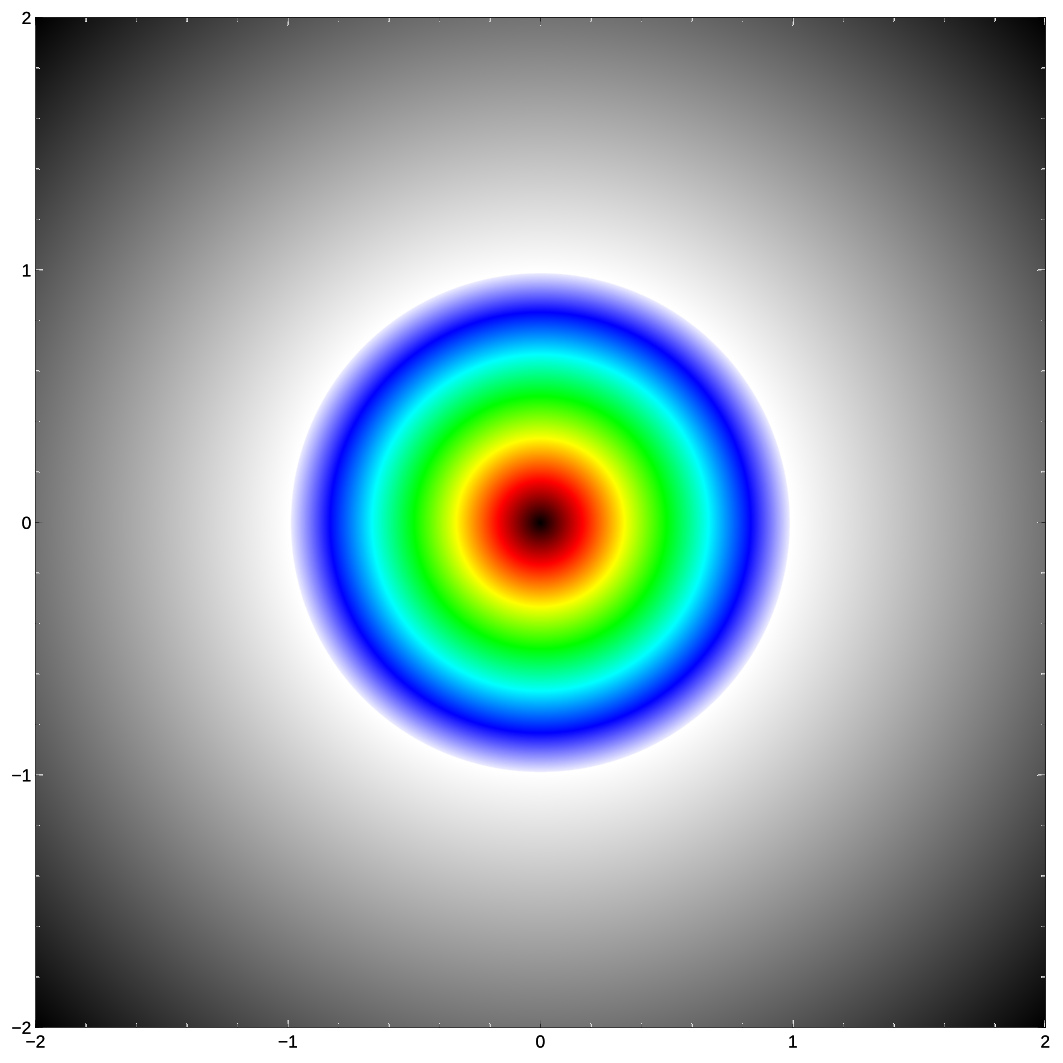
\includegraphics[width=0.5\textwidth, right]{implicit_circle.jpg}
  \end{column}
\end{columns}
\begin{columns}
  \begin{column}{0.5\textwidth}
    \begin{itemize}
    \item $tf(x,y,tx,ty)=sqrt((x-tx)^2+(y-ty)^2)-1$
    \end{itemize}
  \end{column}
  \begin{column}{0.5\textwidth}
    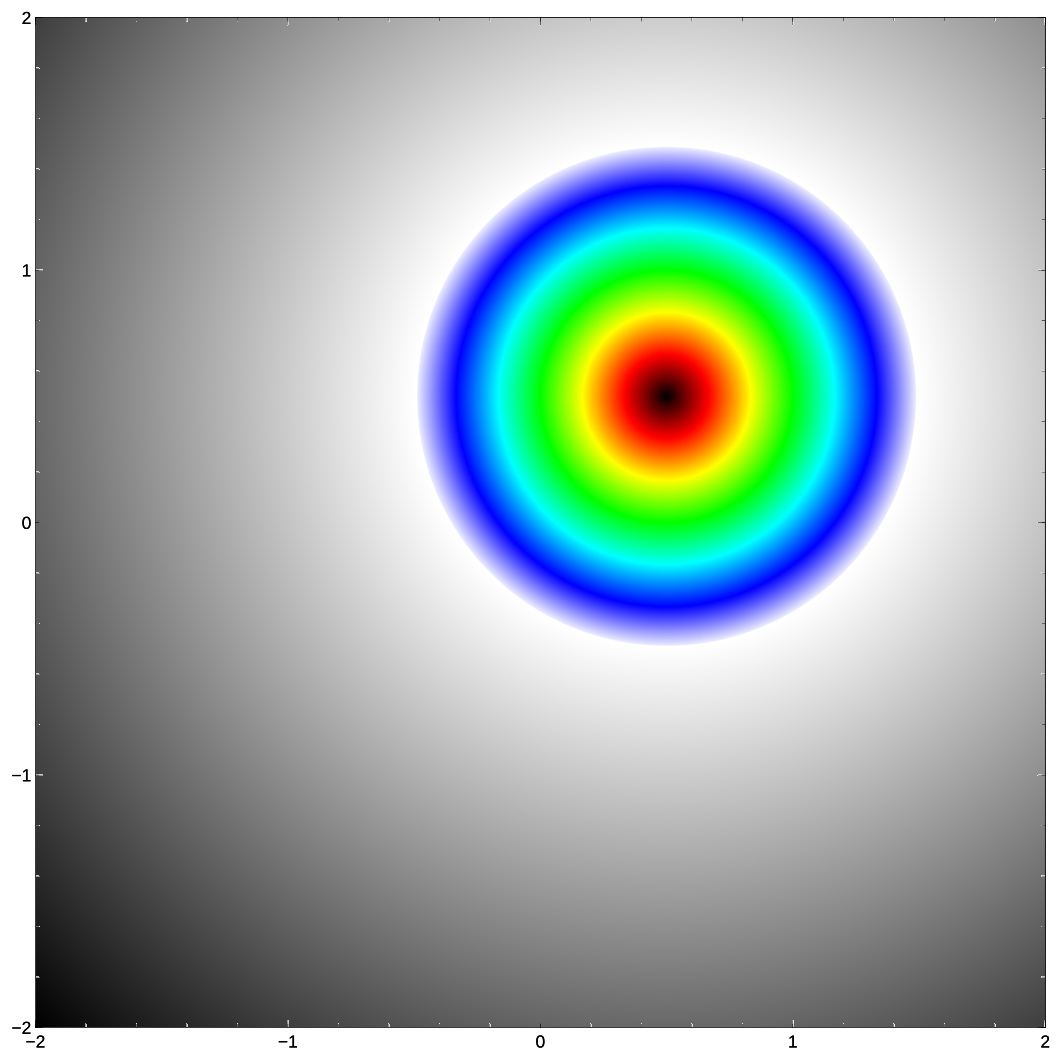
\includegraphics[width=0.5\textwidth, right]{implicit_translated_circle.jpg}
  \end{column}
\end{columns}
\end{frame}

\begin{frame}
\frametitle{Scaling}
\begin{columns}
  \begin{column}{0.5\textwidth}
    \begin{itemize}
    \item $f(x,y)=sqrt(x^2+y^2)-1$
    \end{itemize}
  \end{column}
  \begin{column}{0.5\textwidth}
    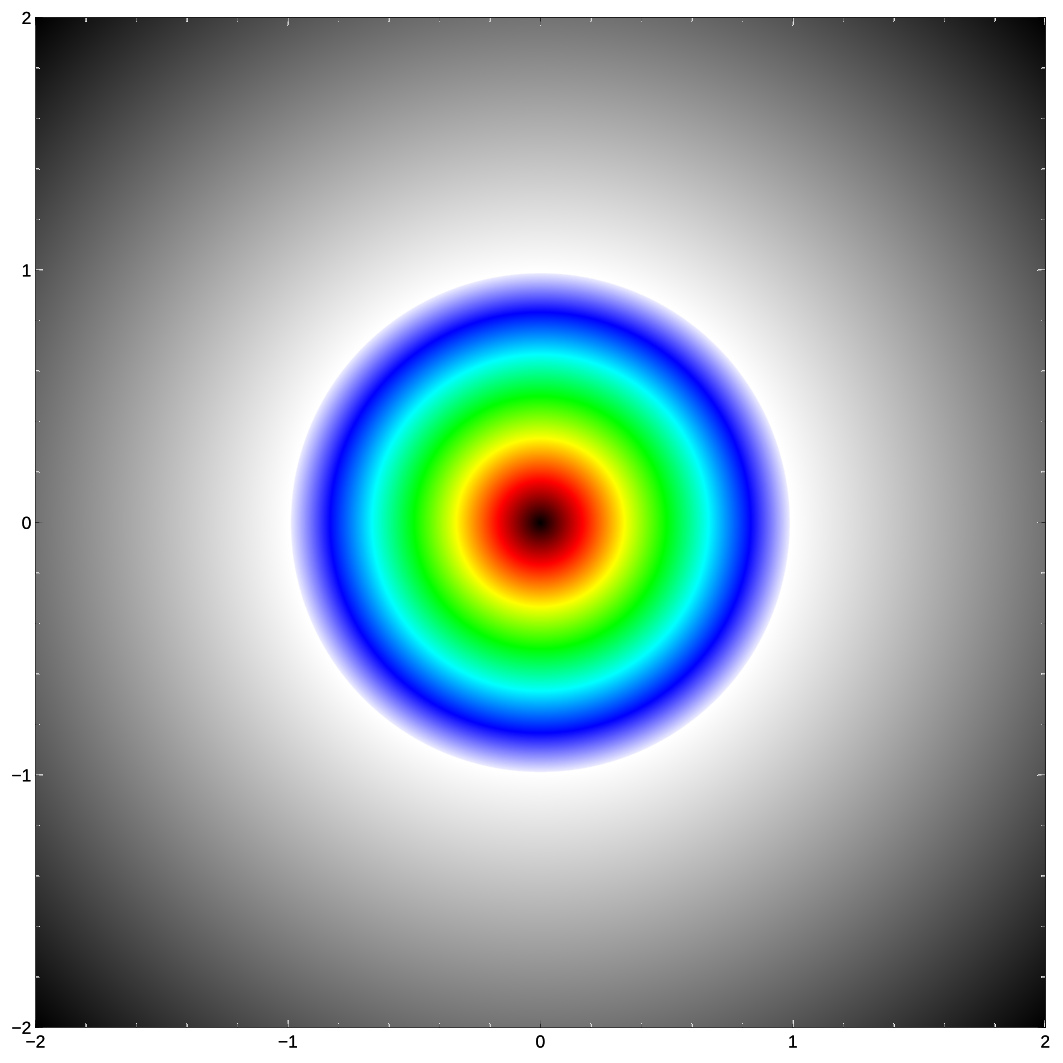
\includegraphics[width=0.5\textwidth, right]{implicit_circle.jpg}
  \end{column}
\end{columns}
\begin{columns}
  \begin{column}{0.5\textwidth}
    \begin{itemize}
    \item $sf(x,y,sx,sy)=sqrt((x/sx)^2+(y/sy)^2)-1$
    \end{itemize}
  \end{column}
  \begin{column}{0.5\textwidth}
    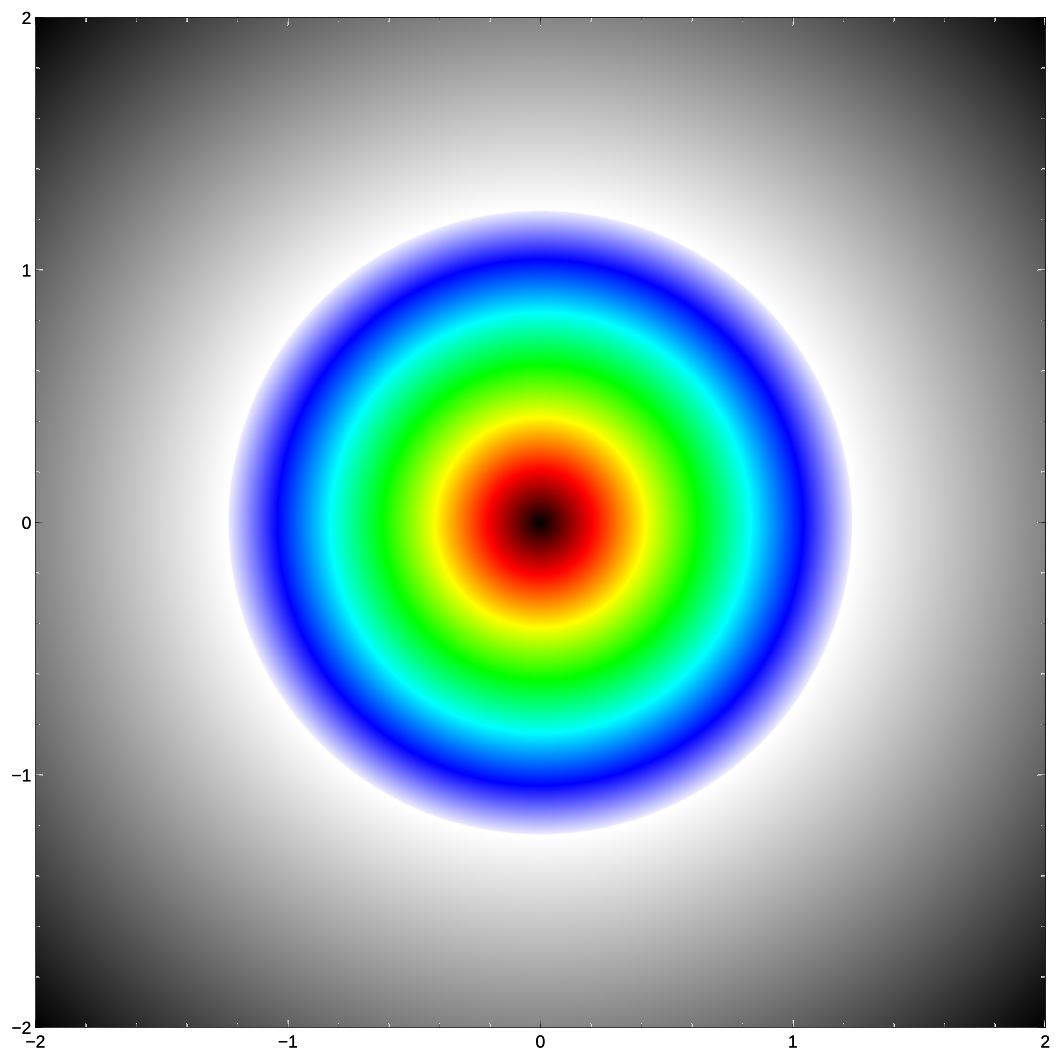
\includegraphics[width=0.5\textwidth, right]{implicit_scaled_circle.jpg}
  \end{column}
\end{columns}
\end{frame}

\begin{frame}
\frametitle{Squares}
\begin{columns}
  \begin{column}{0.75\textwidth}
    \begin{itemize}
    \item $abs(x)=r \land abs(y)<r \lor abs(y)=r \land abs(x)<r$
    \end{itemize}
  \end{column}
  \begin{column}{0.25\textwidth}
    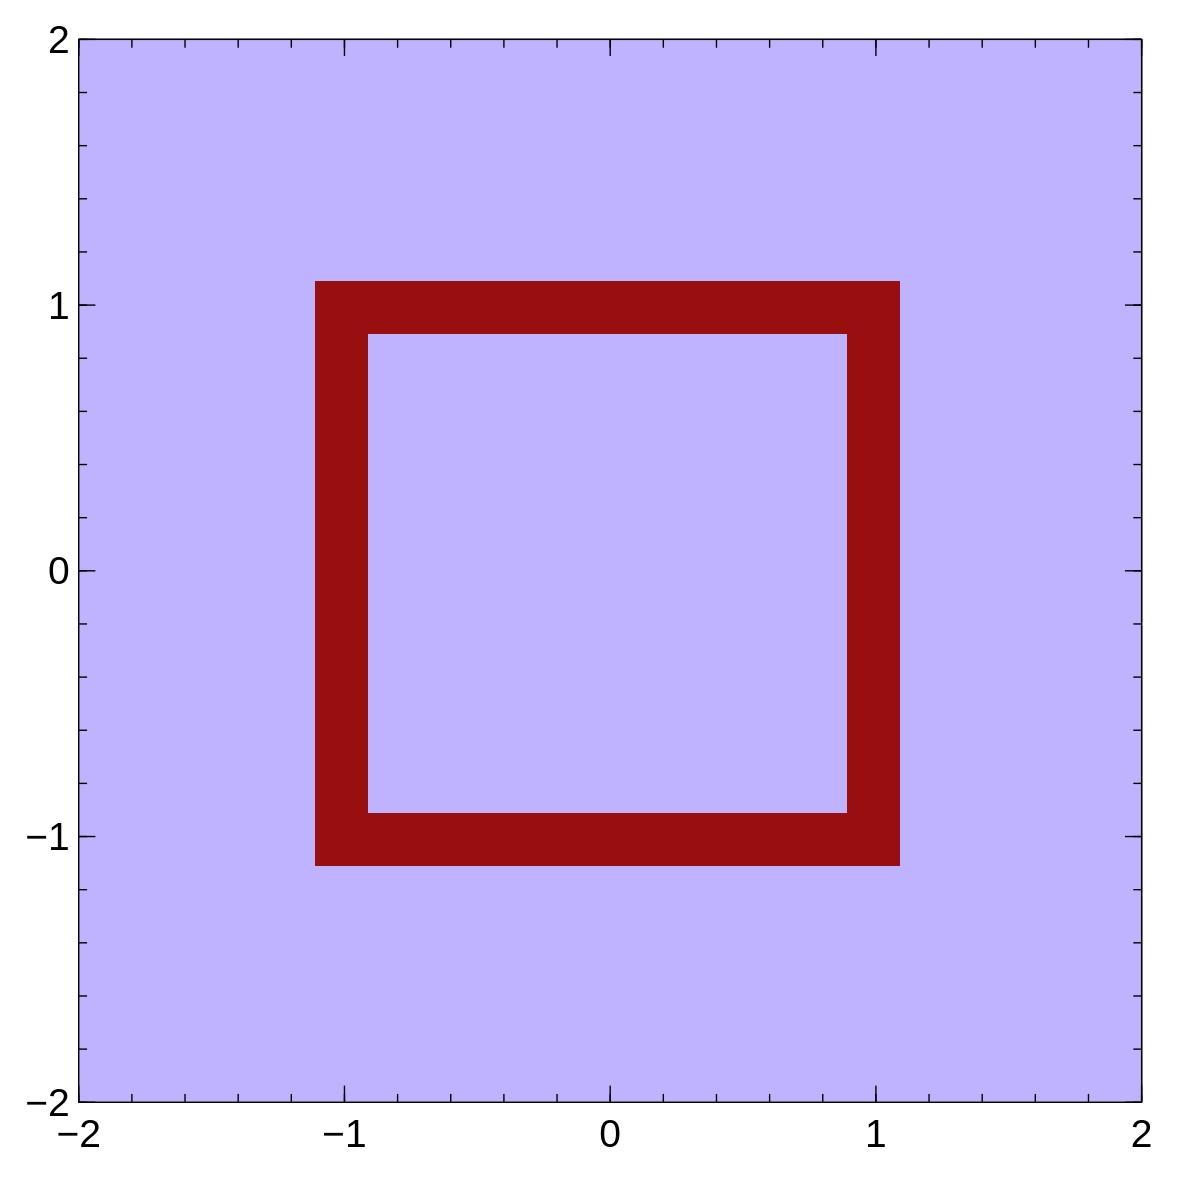
\includegraphics[width=1.0\textwidth, right]{normal_square.jpg}
  \end{column}
\end{columns}
\begin{columns}
  \begin{column}{0.75\textwidth}
    \begin{itemize}
    \item $f(x,y)=maximum(abs(x),abs(y))-1$
    \end{itemize}
  \end{column}
  \begin{column}{0.25\textwidth}
    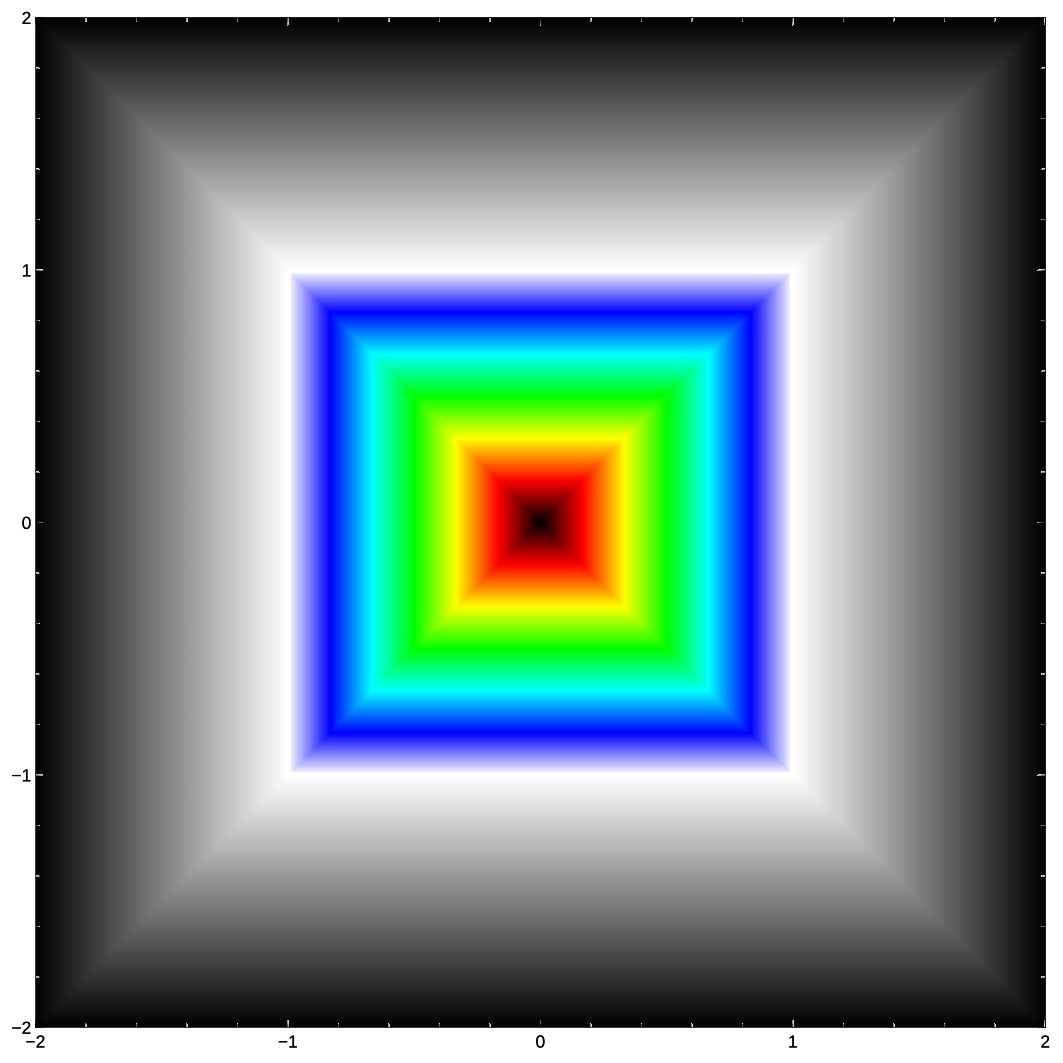
\includegraphics[width=1.0\textwidth, right]{implicit_square.jpg}
  \end{column}
\end{columns}
\end{frame}

\begin{frame}[fragile]
\frametitle{Unioning}
\begin{columns}
  \begin{column}{0.33\textwidth}
  \lstset{basicstyle=\ttfamily\scriptsize}
    \begin{lstlisting}
    f(x,y)=sqrt(x^2+y^2)-1
    f(x,y)=maximum(
      abs(x),abs(y)
      )-1
    \end{lstlisting}
  \end{column}
  \begin{column}{0.60\textwidth}
  \lstset{basicstyle=\ttfamily\scriptsize}
    \begin{lstlisting}
      f(x,y) = minimum(
      sqrt((x+0.25)^2+(y+0.25)^2)-1,
      maximum(abs(x-0.25),abs(y-0.25))-1
      )
    \end{lstlisting}
  \end{column}
\end{columns}
\begin{columns}
  \begin{column}{0.33\textwidth}
    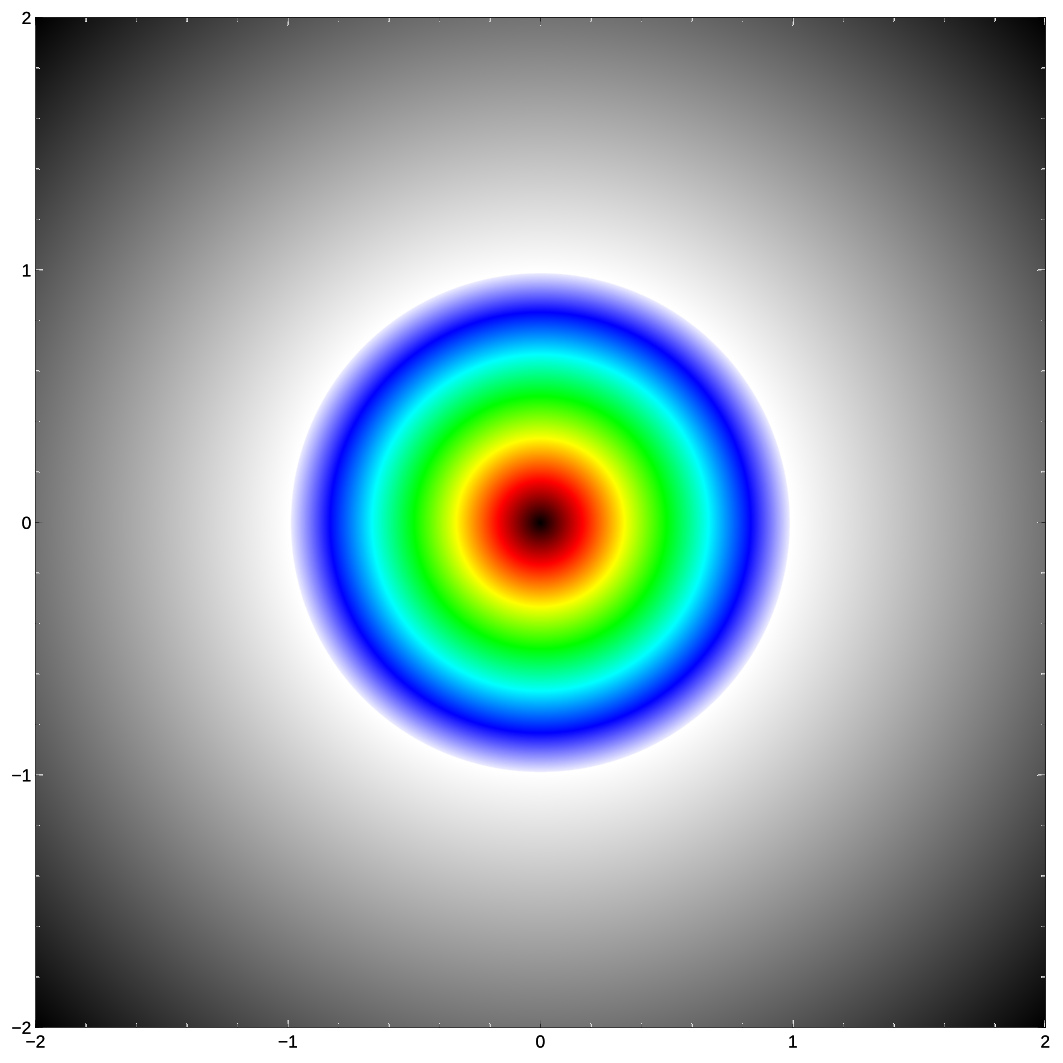
\includegraphics[width=0.9\textwidth, left]{implicit_circle.jpg}
  \end{column}
  \begin{column}{0.33\textwidth}
    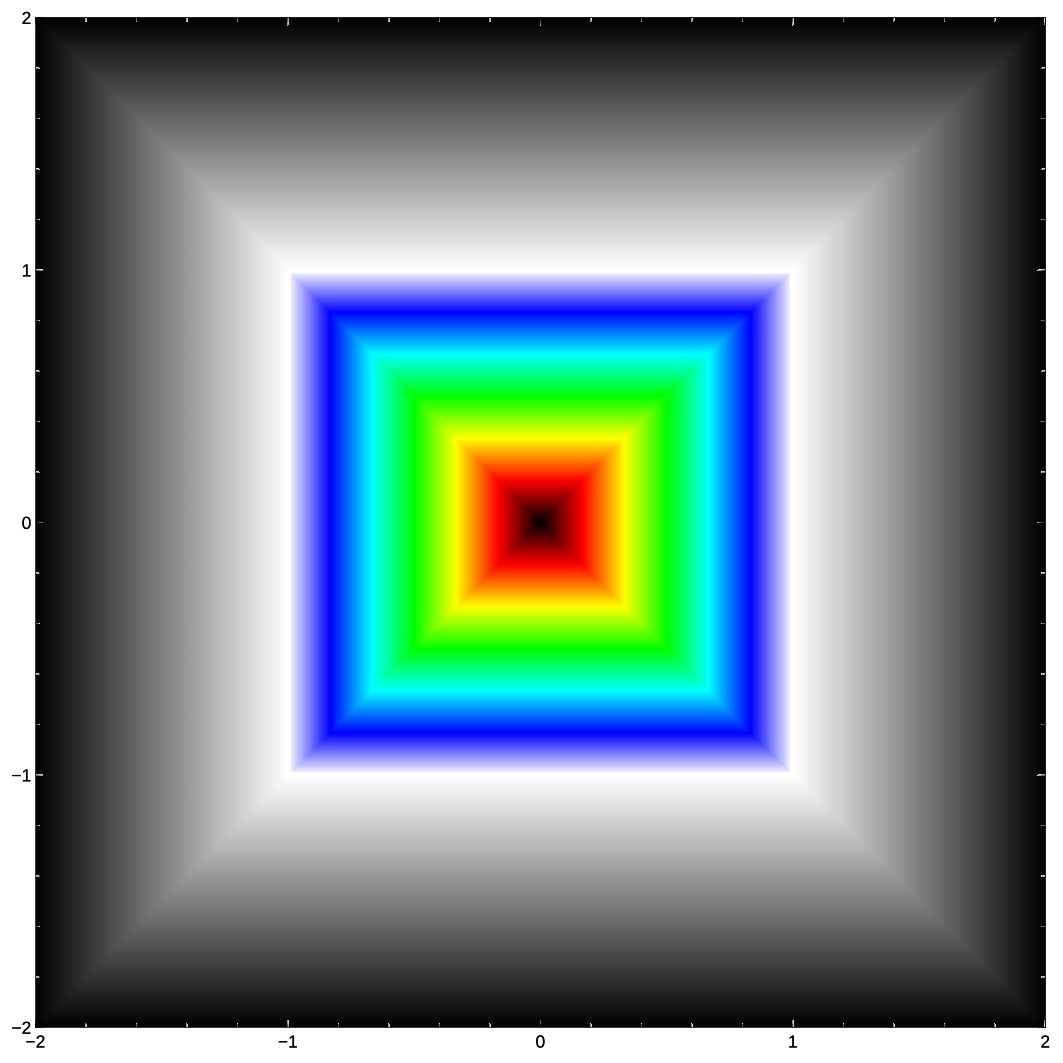
\includegraphics[width=0.9\textwidth, center]{implicit_square.jpg}
  \end{column}
  \begin{column}{0.33\textwidth}
    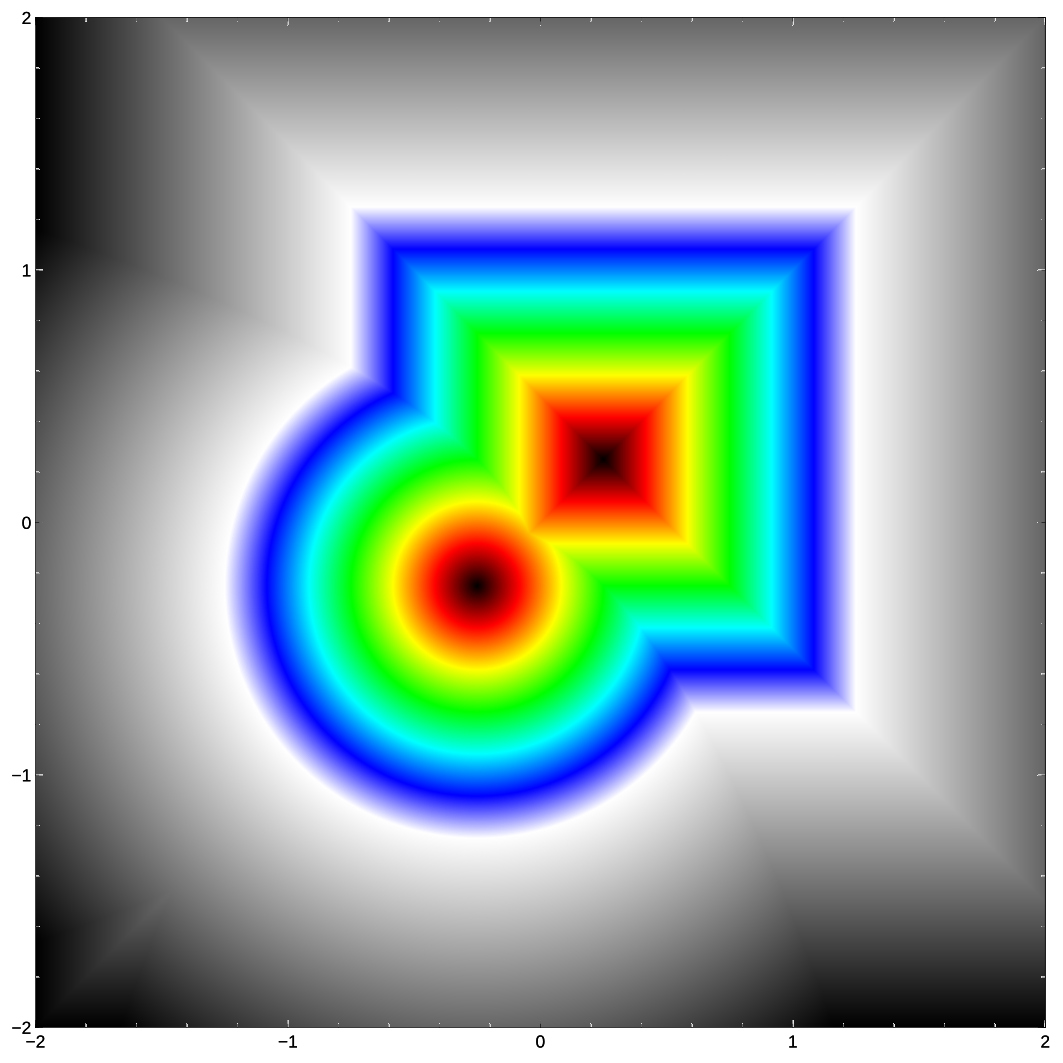
\includegraphics[width=0.9\textwidth, center]{implicit_union_square_circle.jpg}
  \end{column}
\end{columns}
\end{frame}

\begin{frame}[fragile]
\frametitle{Intersecting}
\begin{columns}
  \begin{column}{0.75\textwidth}
    \lstset{basicstyle=\ttfamily\scriptsize}
    \begin{itemize}
    \item Taking the maximum of the two items gives the intersection
    \end{itemize}
    \begin{lstlisting}
      maximum(
        sqrt((x+0.25)*(x+0.25)+(y+0.25)*(y+0.25))-1,
        maximum(abs(x-0.25),abs(y-0.25))-1
        )
    \end{lstlisting}
  \end{column}
  \begin{column}{0.25\textwidth}
    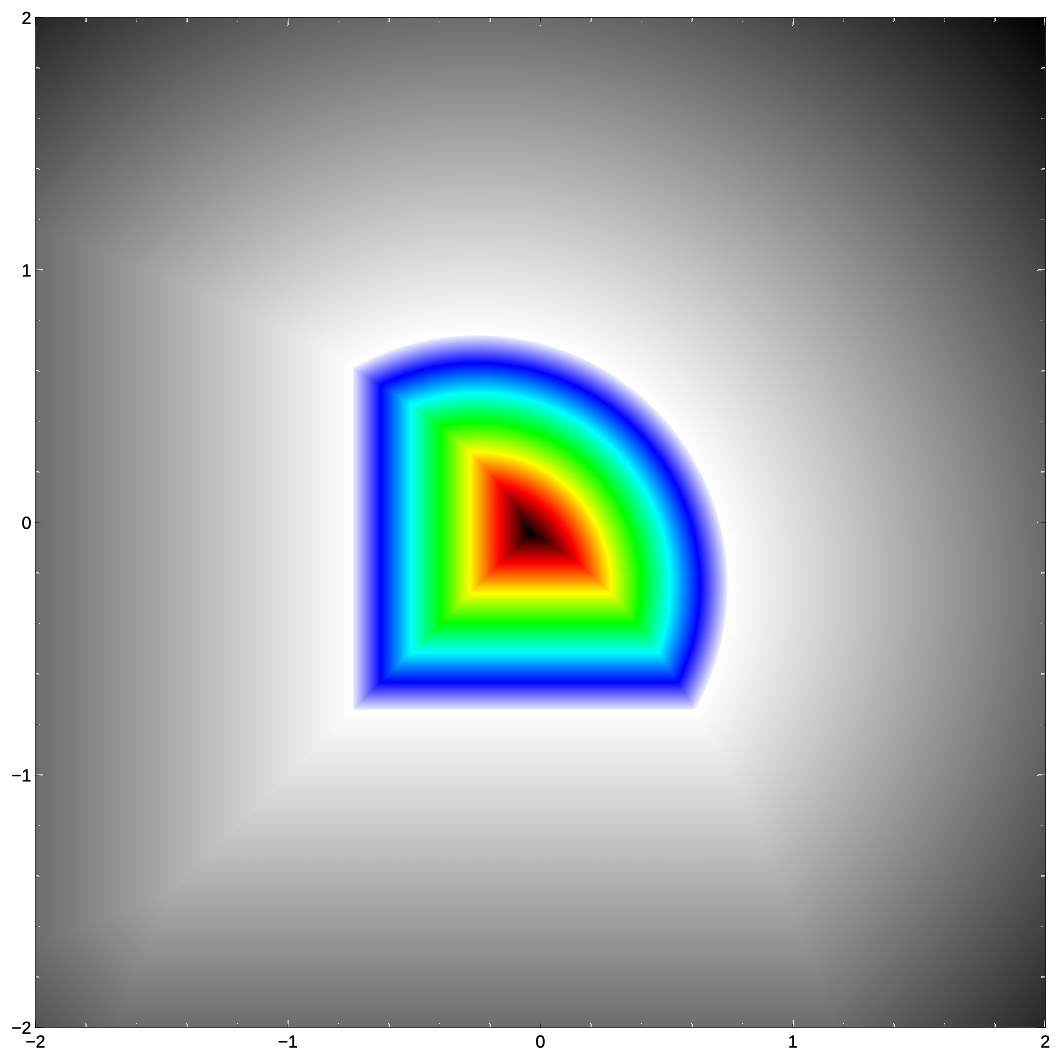
\includegraphics[width=1.0\textwidth, right]{implicit_intersection_square_circle.jpg}
  \end{column}
\end{columns}
\end{frame}

\begin{frame}
\frametitle{Getting the Difference}
\begin{columns}
  \begin{column}{0.65\textwidth}
    \begin{itemize}
    \item Taking the maximum of the item to be removed from, and the inverse of the items being removed gives the difference
    \item $maximum(sqrt((x+0.25)*(x+0.25)+(y+0.25)*(y+0.25))-1,-(maximum(abs(x-0.25),abs(y-0.25)))-1)$
    \end{itemize}
  \end{column}
  \begin{column}{0.35\textwidth}
    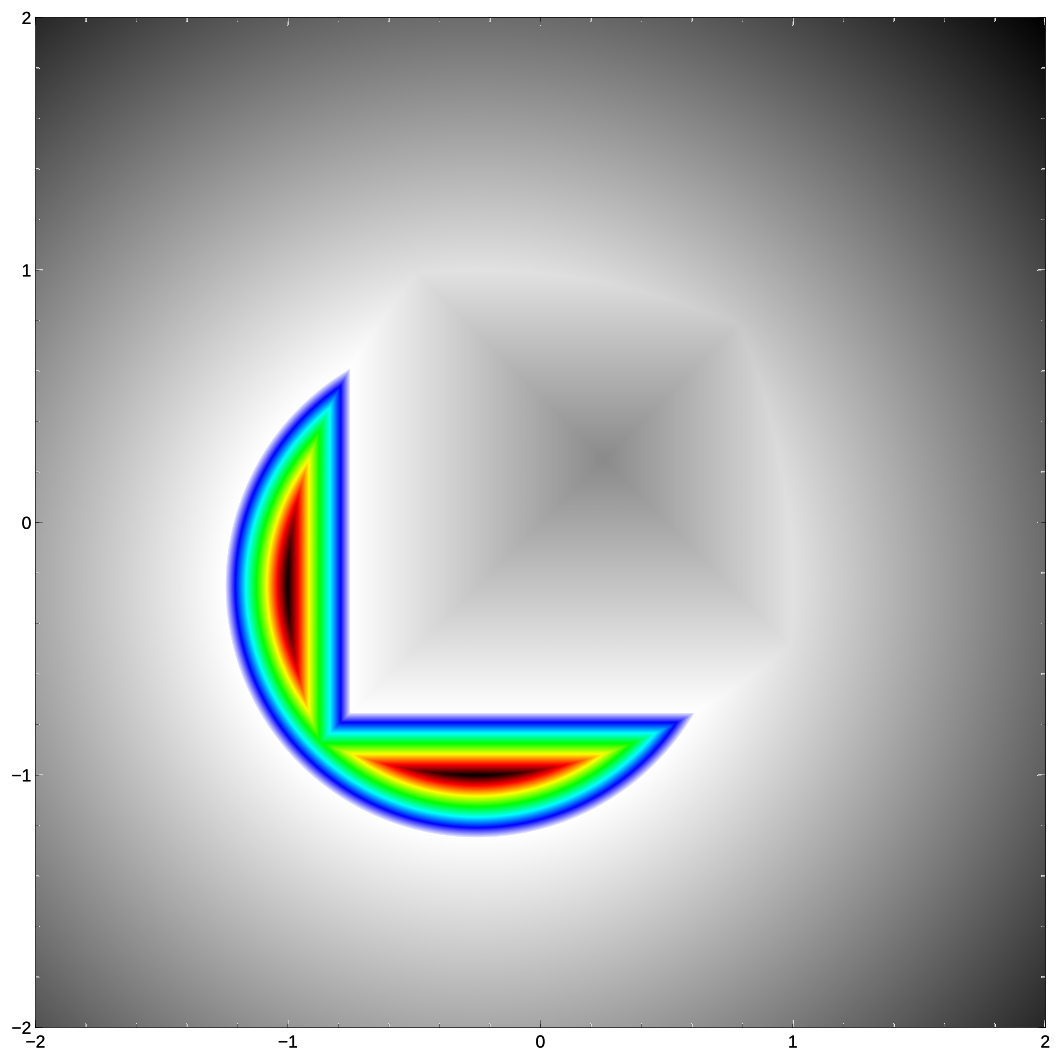
\includegraphics[width=1.0\textwidth, right]{implicit_difference_square_circle.jpg}
  \end{column}
\end{columns}
\end{frame}

\begin{frame}
\frametitle{Rounded Unions}
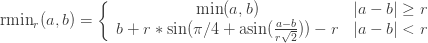
\includegraphics[width=0.8\textwidth, center]{rounded_union_formula.png}
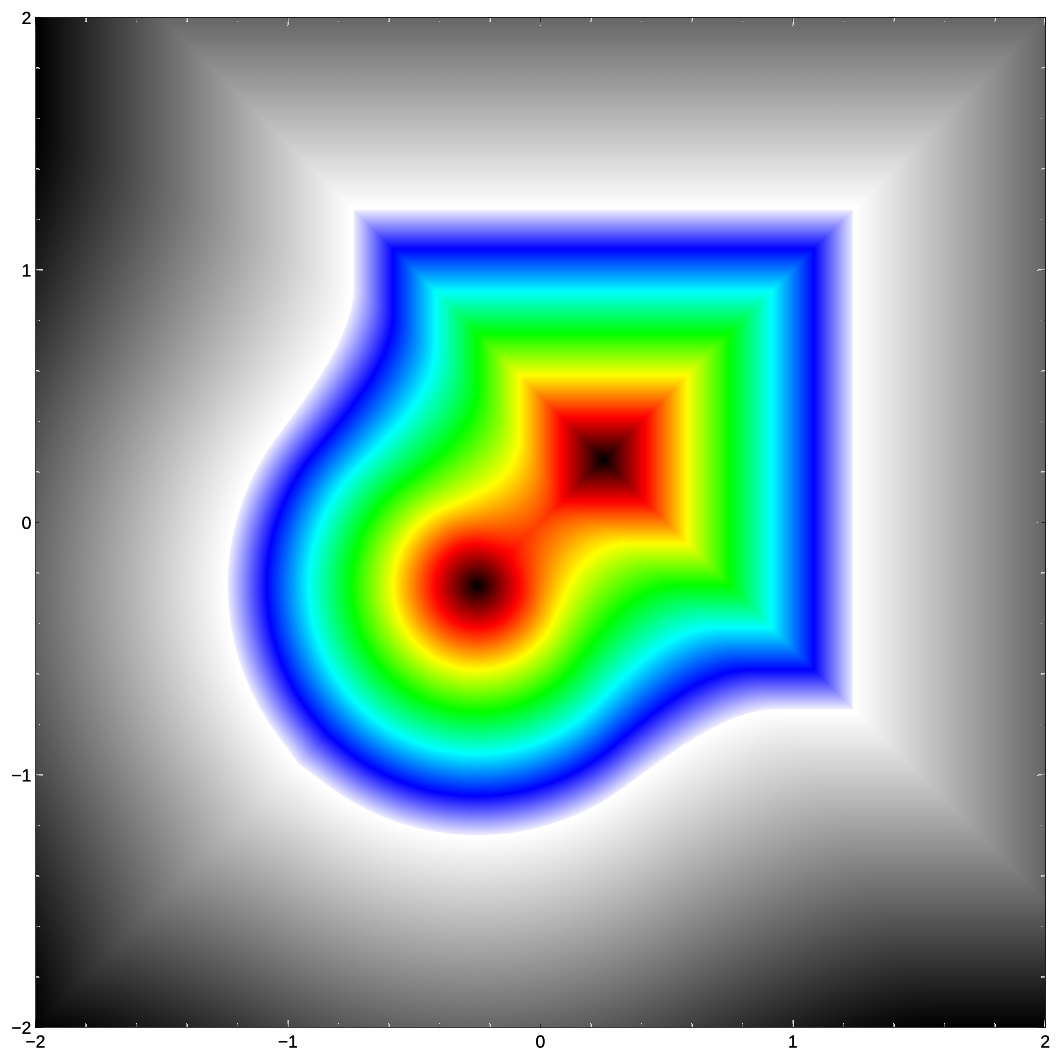
\includegraphics[width=0.6\textwidth, center]{implicit_union_rounded_square_circle.jpg}
\end{frame}

\section{Implicit CSG Implications}

\begin{frame}
\frametitle{Implicit CSG Advantages}
\begin{itemize}
\item Easy Rounding
\end{itemize}
\begin{columns}
  \begin{column}{0.75\textwidth}
    \begin{itemize}
    \item $square (x=30,y=30,r=5)$
    \end{itemize}
  \end{column}
  \begin{column}{0.25\textwidth}
    
\includegraphics[width=1.0\textwidth, right]{website-rounded_square.png}
  \end{column}
\end{columns}
\begin{itemize}
\item $square (x=30,y=30,r=15)$ == Circle!
\item Most primitives support rounding
\item Rendering can be matched to your ability to print
\end{itemize}
\end{frame}

\begin{frame}[fragile]
\frametitle{Implicit CSG Disadvantages}
\begin{itemize}
\item Eats CPU
\item Must track render area, as well as function stack
  \begin{itemize}
  \item Tighter boxes mean less CPU wasted
  \end{itemize}
\end{itemize}
\end{frame}

\section{Haskell Implications}

\begin{frame}[fragile]
  \frametitle{Haskell Implications}
  \begin{itemize}
  \item Can generate and use functions
    \begin{itemize}
    \item Hard to reason about them
    \item Cannot print in intermediate form dump
    \end{itemize}
  \item List comprehensions parallelize well
  \item ... Sadly little overlap between Haskellers and 3D modelers
  \item Always telling users to use ``+RTS -N -qg'' is painful
  \end{itemize}
\end{frame}

\begin{frame}[fragile]
  \frametitle{Using Functions}
      \lstset{basicstyle=\ttfamily\scriptsize}
      \begin{lstlisting}
        linear_extrude (height = 40, twist(h) = 35*cos(h*2*pi/60))
        union ( r = 8) {
          circle (10);
          translate ([22,0]) circle (10);
          translate ([0,22]) circle (10);
          translate ([-22,0]) circle (10);
          translate ([0,-22]) circle (10);
        }
      \end{lstlisting}
      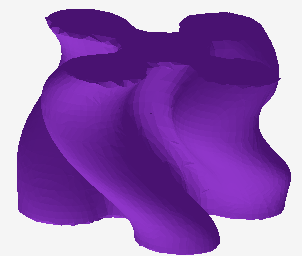
\includegraphics[width=0.5\textwidth, center]{website-example_object.png}
\end{frame}

\begin{frame}[fragile]
\frametitle{linear\_extrude functional arguments}
\begin{itemize}
\item $height(x,y) = value$
\item $twist(h) = value$
\item $scale(h) = value$
\item $translate(h) = (x,y)$
\end{itemize}
\end{frame}

\section{Real World Example}
\begin{frame}
\frametitle{Real World}
\begin{columns}
  \begin{column}{0.5\textwidth}
  \begin{itemize}
  \item My 3D Printer
    \begin{itemize}
    \item LulzBot Taz 3-5ish
    \item Re-printing with ImplicitCAD
    \item STLs provided by LulzBot
      \begin{itemize}
        \item STLs are not source code!
      \end{itemize}      
    \end{itemize}
  \end{itemize}
  \end{column}
  \begin{column}{0.5\textwidth}
\includegraphics[width=0.7\textwidth, center]{my_printer.jpg}
  \end{column}
\end{columns}
\end{frame}

\begin{frame}
\frametitle{Cracking Parts}
\includegraphics[width=0.5\textwidth, center]{my_printer-cracked.jpg}
\end{frame}

\begin{frame}
\frametitle{Stress under Pressure}
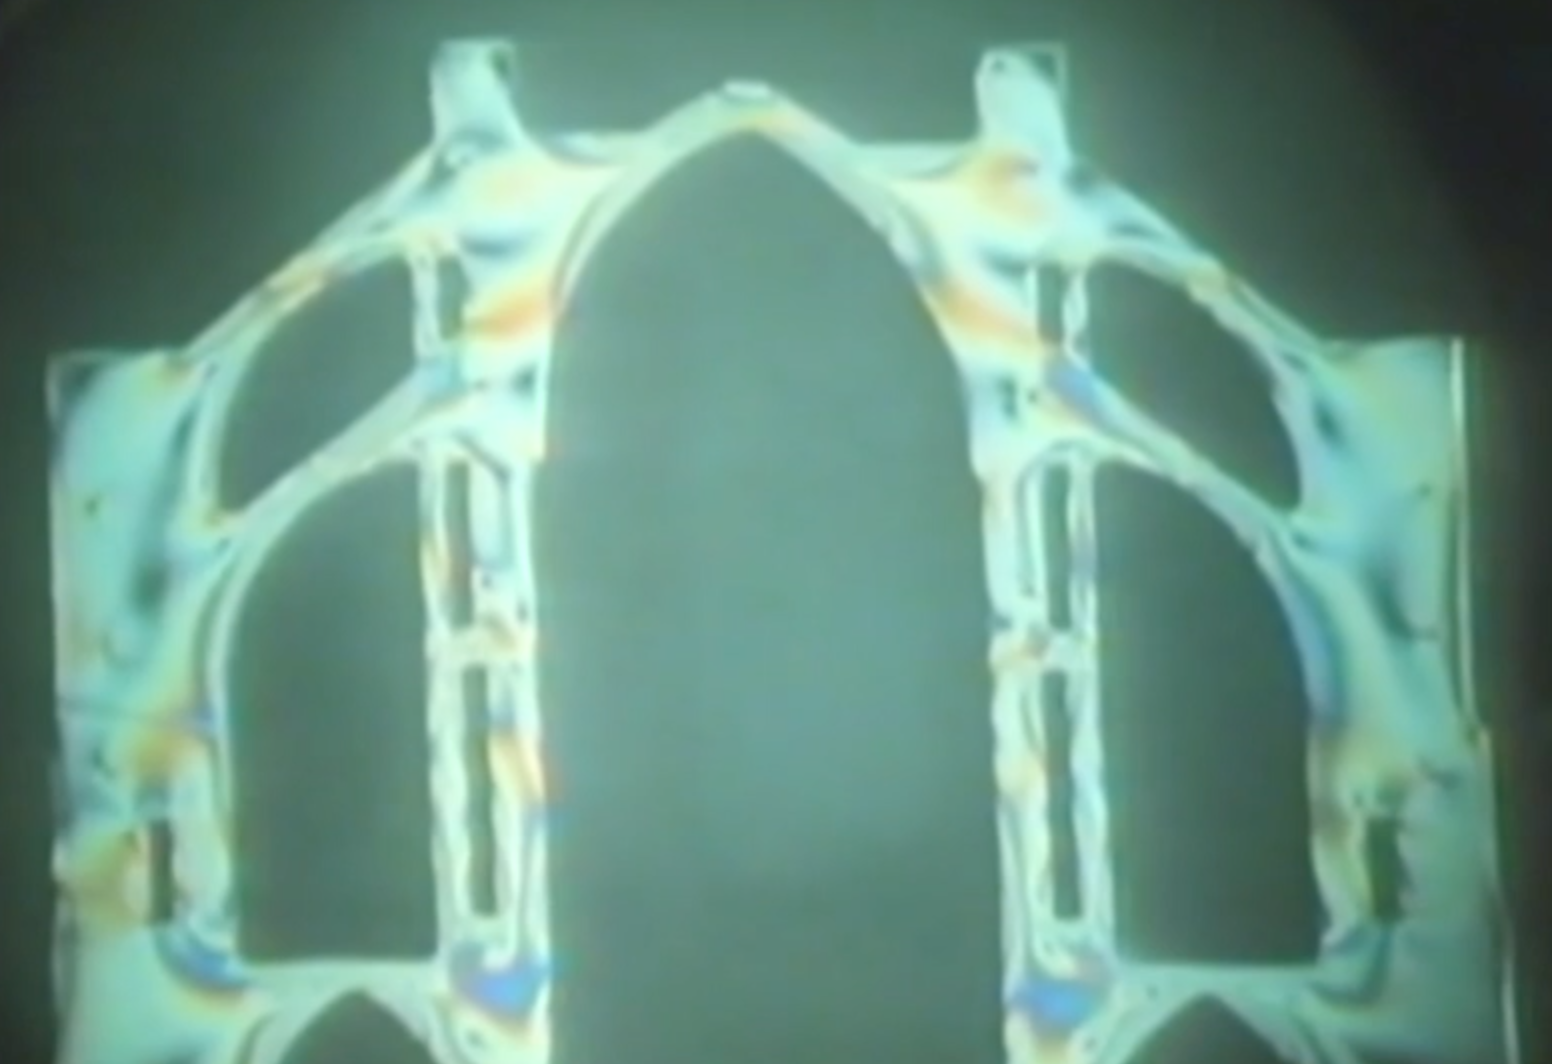
\includegraphics[width=0.7\textwidth, center]{robert_mark-cathedral.png}
\end{frame}

\begin{frame}
\frametitle{Rounding}
\includegraphics[width=0.7\textwidth, center]{cura-bearing_holder.png}
\end{frame}

\section{Future Functionality}
\begin{frame}[fragile]
\frametitle{Future ImplicitCAD Functionality}
\begin{itemize}
\item Functions as a type, so they can be reasoned about by the engine
\item User-defined implicit operations
\end{itemize}
\lstset{basicstyle=\ttfamily\scriptsize}
\begin{lstlisting}
  raw3D(bbox=function_that_returns_two_points,
        implicit(x,y,z)=function_that_returns_a_value);
\end{lstlisting}
\end{frame}

\section{Other Software}

\begin{frame}
  \frametitle{What is HSlice?}
\begin{itemize}
\item Another Slicer!
\item Originally written by Catherine Moresco and Noah Halford in 2016
  \begin{itemize}
  \item I took over as lead developer last year
  \end{itemize}
\item Licensed under the AGPLv3+
\item Written in Haskell
\item Goals:
  \begin{itemize}
  \item Support slicing for printers with combined linear and rotational motion
  \item Part of my effort to have a 100 percent haskell based 3D printing stack 
  \end{itemize}
\item Abuses the expression evaluation from ImplicitCAD..
\end{itemize}
\begin{block}{Source Code}
\begin{itemize}
\item https://github.com/julialongtin/HSlice/
\end{itemize}
\end{block}
\end{frame}

\begin{frame}
\frametitle{Functional OpenSCAD}
\includegraphics[width=0.7\textwidth, center]{openscad-functional.png}
\end{frame}

\begin{frame}
  \frametitle{ExplicitCAD}
\begin{itemize}
\item A graphical front end for ImplicitCAD
\item Originally written by Kliment
\item Licensed under the GPLv3
\item Written in C++
\item Goals:
  \begin{itemize}
  \item Give ImplicitCAD a better look and feel for non-command line users
  \end{itemize}
\end{itemize}
\begin{block}{Source Code}
\begin{itemize}
\item https://github.com/kliment/explicitcad
\end{itemize}
\end{block}
\end{frame}

\begin{frame}
\frametitle{-Fin-}
\Huge{\centerline{Questions?}}
\end{frame}

%----------------------------------------------------------------------------------------

\end{document} 
